\documentclass[a4paper]{article} % Create new a report
\usepackage[utf8]{inputenc}
\usepackage[T5]{fontenc} % To use unicode
\usepackage{mathptmx} % Time New Roman
\usepackage[right=2cm,left=3cm,top=2cm,bottom=2.5cm]{geometry}
\usepackage[fontsize=13pt]{scrextend}
\usepackage{graphicx} % Required for inserting images
\usepackage{indentfirst}
\usepackage{float} % Set position of image.
\usepackage{tikz} % Create border
\usepackage{multicol}
\usepackage{caption}
\usepackage{array} % Required for Table Column Text Alignment with Custom Widths
\usepackage{titlesec} % Set font style
\usepackage{parskip}
\usepackage{xcolor}
\usepackage{listings}
\usepackage{tocloft}
\usepackage{xparse}
\usepackage{forloop}
\usepackage{enumitem}
\usepackage{lipsum}
\usepackage{textcase}
\usepackage{tabularray}
\usepackage{longtable}
\usepackage{changepage}
\usepackage[inkscape = inkscape -z -D, svgpath = fig/]{svg}

\usetikzlibrary{calc}
%Custom packages
\usepackage{./config/heading}
\usepackage{./config/fancy}
\usepackage{./config/figure}

\setlist{nolistsep}
\renewcommand{\baselinestretch}{1.2}
\setlength{\parskip}{6pt} % Spacing after
\setlength{\parindent}{1cm}

\newcommand{\setsection}[1]{\section*{\texorpdfstring{\MakeTextUppercase{#1}}{#1}}\addcontentsline{toc}{section}{\texorpdfstring{\MakeTextUppercase{#1}}{#1}}\markright{#1}}
\newcommand{\setsubsection}[1]{\subsection*{\texorpdfstring{\MakeTextUppercase{#1}}{#1}}\addcontentsline{toc}{subsection}{\texorpdfstring{\MakeTextUppercase{#1}}{#1}}\markright{#1}}


% Link to figure
\usepackage[unicode]{hyperref}
\newcommand{\myref}[1]{\textbf{\hyperref[#1]{Hình~\ref*{#1}}}}
\newcommand{\myreftb}[1]{\textbf{\hyperref[#1]{Bảng~\ref*{#1}}}}

\DefTblrTemplate{contfoot-text}{default}{Tiếp tục bên trang tiếp theo}
\DefTblrTemplate{conthead-text}{default}{(Tiếp tục)}

% =========================== START DOCUMENT ==================================
\begin{document}

\pagenumbering{roman} % Đánh số thứ tự la mã
% \begin{titlepage}
  \begin{tikzpicture}[overlay, remember picture]
    \draw [line width=3pt]
    ($ (current page.north west) + (3.0cm,-2.0cm) $)
    rectangle
    ($ (current page.south east) + (-2.0cm,2.5cm) $);
    \draw [line width=0.5pt]
    ($ (current page.north west) + (3.1cm,-2.1cm) $)
    rectangle
    ($ (current page.south east) + (-2.1cm,2.6cm) $);
  \end{tikzpicture}
  \begin{center}
    \vspace{-6pt}TRƯỜNG ĐẠI HỌC CẦN THƠ \\
    \textbf{\fontsize{16pt}{0pt}\selectfont TRƯỜNG CÔNG NGHỆ THÔNG TIN VÀ TRUYỀN THÔNG}
    % \vspace{0.5cm}
    \begin{figure}[H]
      \centering
      
\includegraphics[width=5cm]{images/logo-ctu.png}
    \end{figure}
    \textbf{Phát triển ứng dụng Web} \\
    \textbf{Mã Học Phần: CT449} \\
    \textbf{Nhóm học phần: 03} \\
    \vspace{3.5cm}
    \textbf{\fontsize{16pt}{0pt}\selectfont BÁO CÁO} \\
    \textbf{\fontsize{18pt}{0pt}\selectfont XÂY DỰNG WEBSITE MƯỢN SÁCH} \\
    \vspace{4.5cm}
    \newcommand{\MyIndent}{\hspace{1cm}}
    \begin{tabular}{p{8cm} l}
      \textbf{Giáo viên hướng dẫn}        & \textbf{Sinh viên thực hiện}  \\
      \MyIndent ThS.GVC Nguyễn Minh Trung & \MyIndent Tên: Nguyễn Tuấn Đạt \\
                                          & \MyIndent MSSV: B2203499
    \end{tabular}


    \vspace{2cm}
    \fontsize{14pt}{0pt}\selectfont Học Kỳ II, 2023 - 2024
  \end{center}
\end{titlepage}
\cleardoublepage


% \section*{LỜI CẢM ƠN}
Trong suốt quá trình thực hiện bài tập lớn, em xin gửi một lời cảm ơn chân thành những người đã giúp đỡ, hỗ trợ tận tình cho em hoàn thành bài tập này. \par
Đầu tiên, em muốn bày tỏ lòng biết ơn sâu sắc đến giảng viên hướng dẫn của mình, Thầy Nguyễn Minh Trung. Với việc giảng dạy, hỗ trợ tận tâm, Thầy đã giúp em vượt qua những khó khăn trong quá trình học tập và hoàn thiện bài tập. Sự hướng dẫn, chỉ dạy từ Thầy không chỉ giúp em hiểu sâu hơn về các công nghệ như Vue.js, MongoDB, và Express mà còn hướng dẫn cho em khả năng tự học, đọc tài liệu và liên tục cập nhật các thay đổi mới nhất về công nghệ xây dựng website. \par
Trải qua những giờ phút nỗ lực, học hỏi không ngừng nghĩ, em cũng đã nhận ra niềm vui, nhận ra sự yêu thích lập trình, đặc biệt là về mảng lập trình web, cũng đã tự hào vì đã có thể hoàn thành bài tập này một cách tâm huyết nhất và hoàn thiện nhất.\par
Không thể không đề cập đến sự giúp đỡ và hỗ trợ từ bạn bè. Những người đã tận tình giúp đỡ em vượt qua những khó khăn vấp phải khi lập trình và trình bày báo cáo
. \par
Một lần nữa, em xin chân thành cảm ơn tất cả mọi người.
\vspace{6pt}
\hspace{7cm}Cần Thơ, ngày 24 tháng 04 năm 2024

\hspace{9cm}\textbf{Sinh viên thực hiện}

\vspace{2cm}
\hspace{9.25cm}\textbf{Nguyễn Tuấn Đạt}
\thispagestyle{empty}
\newpage


% \addtocontents{toc}{\protect\thispagestyle{empty}}
\renewcommand{\contentsname}{MỤC LỤC}
\tableofcontents
\thispagestyle{empty}
\cleardoublepage

\pagenumbering{roman}
% ======= SET UP LIST OF FIGURES =======
\setlength{\cftfigindent}{0pt}
\setlength{\cftfignumwidth}{4em}
\renewcommand{\cftfigdotsep}{1.5}
\renewcommand{\figurename}{\fontsize{12pt}{0pt}\selectfont Hình}
\renewcommand{\thefigure}{\thesection.\arabic{figure}}
\renewcommand{\cftfigpresnum}{\figurename~}
\renewcommand{\listfigurename}{DANH MỤC HÌNH}
\phantomsection
\addcontentsline{toc}{section}{DANH MỤC HÌNH}
\listoffigures
\cleardoublepage

% ======= SET UP LIST OF TABLES =======
\setlength{\cfttabindent}{0pt}
\setlength{\cfttabnumwidth}{4em}
\renewcommand{\cfttabdotsep}{1.5}
\renewcommand{\tablename}{\fontsize{12pt}{0pt}\selectfont Bảng}
\renewcommand{\cfttabpresnum}{\tablename~}
\renewcommand{\listtablename}{DANH MỤC BẢNG}
\phantomsection
\addcontentsline{toc}{section}{DANH MỤC BẢNG}
\listoftables
\cleardoublepage






% \section*{DANH MỤC KÝ HIỆU VÀ CHỮ VIẾT TẮT}
% \phantomsection \addcontentsline{toc}{section}{DANH MỤC KÝ HIỆU VÀ CHỮ VIẾT TẮT}
% \begin{longtblr}[ label=none,entry=none,]{  row{1}={font=\bfseries,c}, hlines,vlines,colspec={X[1,c]X[2,c]X[2,c]}}
%   STT & Ký hiệu chữ viết tắt & Chữ viết đầy đủ \\
%   1   & VĐV                  & Vận động viên   \\
%   2   & HLV                  & Huấn luyện viên \\
%   3   & CSVC                 & Cơ sở vật chất
% \end{longtblr}
% \thispagestyle{empty}
% \newpage

\pagenumbering{arabic}
%\phantomsection
\setsection{Chương 1: Giới thiệu}
\setcounter{section}{1}

\phantomsection
\subsection{Đặt vấn đề}
Trong thế giới hiện đại đang phát triển với tốc độ chóng mặt của công nghệ thông tin và phần mềm, việc áp dụng chúng vào mọi lĩnh vực của cuộc sống không chỉ là một xu hướng mà còn là một bước tiến quan trọng để nâng cao hiệu quả và tiện ích cho cả xã hội. Từ việc quản lý thông tin cá nhân đến quản lý doanh nghiệp, xu hướng thương mại điện tử tăng cao,  công nghệ thông tin đang trở thành trái tim của mọi hoạt động.\par
Trong lĩnh vực quản lý cho thuê mượn sách, việc tận dụng công nghệ để xây dựng một hệ thống quản lý thông minh và hiệu quả là điều không thể phủ nhận. Điều này không chỉ giúp cho việc quản lý sách và độc giả trở nên dễ dàng hơn mà còn mở ra những cánh cửa mới cho trải nghiệm người dùng.\par
Bằng cách tạo ra trang web quản lý mượn sách và trang web mượn sách trực tuyến cho đọc giả, chúng ta không chỉ đơn thuần là tạo ra một công cụ quản lý mà còn là một nguồn cảm hứng và khích lệ cho sự phát triển của văn hóa đọc. Tính năng quản lý tài khoản, nhà xuất bản, sách, theo dõi mượn sách của tác giả, giúp người thủ thư có thể dễ dàng theo dõi và quản lý việc mượn sách của đọc giả. Đọc giả cũng có thể dễ dàng thực hiện các thao tác mượn sách và theo dõi lịch sử mượn sách của mình.\par
So với việc quản lý mượn sách và đăng ký mượn sách truyền thống, việc xây dựng một hệ thống quản lý mượn sách thông minh không chỉ là một cách tiết kiệm thời gian và chi phí mà còn là một cơ hội để tạo ra một cộng đồng đam mê sách phát triển và sôi động hơn. Điều này đồng nghĩa với việc mở ra những cánh cửa mới cho việc truyền bá tri thức và phát triển cá nhân.


\phantomsection
\subsection{Mục tiêu đề tài}
Đầu tiên, Tạo ra một website giúp các nhân viên cửa hàng sách, hoặc thư viện quản lý việc mượn sách của các đọc giả một cách dễ dàng, tiện lợi 
.\par
\begin{itemize}[align=left, leftmargin=2cm]
  \item[\textbf{-- Về giao diện và trải nghiệm người dùng (UI/UX)}]:
Giao diện đơn giản, hiện đại với màu trắng xanh là chủ đạo. Thiết kế phù hợp công việc quản lý. Đem lại trải nghiệm tuyệt vời cho người quản lý với việc thực hiện các theo dõi mượn sách, quản lý tài khoản đọc giả và quản lý sách thuận lợi với các thao tác đơn giản dễ dàng sử dụng và các hiệu ứng chuyển trang mượt mà đem lại cảm giác dễ chịu và thoải mái cho người dùng \par
  \item[\textbf{-- Về quản lý}]:
việc xây dựng cơ sở dữ liệu với logic chặt chẽ  giúp tối ưu hóa khả năng quản lý, các thông tin tài khoản người dùng bảo mật chặt chẽ và trách tình trạng rò rõ các dữ liệu quan trọng người dùng. Hệ thống  phân quyền người dùng dựa trên vai trò của họ, trong website quản lý chỉ có người quản lý mới có thể đăng nhập và thực hiện các tác vụ quản lý.  \par
\end{itemize}

Thứ hai, Tạo ra một website bán sách với các tính năng tuyệt vời để các cửa hàng sách hoặc thư viện tiếp cận các đọc giả đồng, đồng thời việc tạo ra một website có thể giúp cửa hàng quảng bá, tiếp thị sách một cách hiệu quả với chi phí duy trì thấp nhưng các tiện ích và tiềm năng là rất lớn cho sự phát triển của cửa hàng và cộng đồng người đọc sách.\par
\begin{itemize}[align=left, leftmargin=2cm]
  \item[\textbf{-- Về giao diện và trải nghiệm người dùng (UI/UX)}]:
giao diện đẹp và hiện đại với màu xanh lục đậm và màu trắng đây là 2 màu sách đem lại sự dễ chịu cho người dùng đồng thời nó cũng toát lên vẻ hiện đại. với bố cục website hài hoài hợp lý giúp người dùng có cái nhìn đặc biệt về website  điều này mang lại hiệu quả cho việc tiếp cận và quảng bá của hàng cũng như tiếp thị các sản phẩm mới đến đọc giả. \par
  \item[\textbf{-- Về hiệu năng hệ thống}]:
việc tối ưu  hệ thống giúp các thao tác người dùng thực hiện trên website có thể diễn ra một cách nhanh chóng tạo cảm giác dễ chịu cho người dùng. Kiểm tra chặt chẽ giúp ngăn chặn việc hệ thống phát sinh các lỗi không đáng có gây cảm giác khó chịu cho người dùng \par
\end{itemize}

\phantomsection
\subsection{Đối tượng và phạm vi nghiên cứu}
Website mượn sách trực tuyến là một trong những nền tảng quan trọng giúp người đọc tiếp cận với hàng ngàn tựa sách một cách thuận tiện và linh hoạt. Đối tượng của nghiên cứu này bao gồm cả người đọc, các thư viện, cửa hàng sách. Mục tiêu của nghiên cứu là tối ưu hóa trải nghiệm người dùng thông qua việc cải thiện giao diện và quy trình mượn sách, đồng thời tối ưu hóa hệ thống quản lý sách để đảm bảo nguồn sách luôn được cập nhật và phân phối một cách hiệu quả. Đọc giả khi có tài khoản thì có thể truy cập trang web thực hiện các tác vụ mượn sách. Riêng nhân viên quản lý với tài khoản riêng của mình có thể hiện các tác vụ quản lý tài khoản, sách, nhà xuất bản và quản lý việc mượn sách\par

\phantomsection
\subsection{Phương pháp nghiên cứu}
\begin{itemize}[label={-}]
    \item Thu nhập các thông tin từ các cửa hàng thương mại trực tuyến sẵn có như shopee, Lazada,.. và cửa hàng bán sách trực tuyến hiện có và sao đó lên ý tưởng.
    \item Tổng hợp các kiến thức về tổ chức, phân tích, thiết kế cơ sở dữ liệu và ngôn ngữ mô hình hóa UML.
    \item Tìm hiểu và sử dụng các công nghệ xây dựng website: vue js,  bootstrap 5, express, mongoose, mongodb,  jwt, ant design.
    \item Nắm vững các kỹ năng lập trình backend, frontend và thiết kế giao diện, thiết kế hệ thống.
\end{itemize}

\phantomsection
\subsection{Các chức năng chính}
Website quản lý cho mượn sách được tạo ra nhằm giúp người quản lý dễ dàng trong việc quản lý việc cho mượn sách, tra cứu được thời gian cho mượn và thời gian trả của từng cuốn sách. \par
Đối với người mượn sách có thể dễ dàng tìm kiếm các cuốn sách hiện có và đặt mượn một cách trực tuyến.

\begin{itemize}[align=left, leftmargin=2cm]
  \item[\textbf{-- Đối với quản trị viên}]:
        \begin{itemize}[label={+}]
          \item Đăng nhập, đăng xuất.
          \item Quản lý tài khoản (Thêm, sửa và xóa tài khoản đọc giả).
          \item Quản lý sách (Thêm, sửa và xóa sách).
          \item Quản lý nhà xuất bản (Thêm, sửa, và xóa nhà xuất bản).
          \item Quản lý mượn sách (Thêm, sửa và xóa lịch sử mượn sách).
        \end{itemize}
  \item[\textbf{-- Đối với đọc giả}]:
        \begin{itemize}[label={+}]
          \item Đăng nhập, đăng xuất, tạo tài khoản.
          \item Xem danh sách sản phẩm.
          \item Quản lý thông tin cá nhân: xem và chỉnh sửa thông tin cá nhân. cho sách)
          \item Tìm kiếm sách.
          \item Xem mô tả chi tiết sách.
          \item Mượn sách.
        \end{itemize}
\end{itemize}

%\phantomsection
\setsection{Chương 2: Đặc tả yêu cầu}
\setcounter{section}{2}
\setcounter{subsection}{0}

\phantomsection

\subsection{Mô tả bài toán}
Tạo ra một trang web quản lý mượn sách nhằm đáp ứng nhu cầu mượn sách của người dùng một cách thuận tiện và tiết kiệm thời gian, giảm bớt sự cần thiết phải đến trực tiếp nơi mượn sách để kiểm tra sự có mặt của cuốn sách mong muốn. Người dùng chỉ cần truy cập vào trang web và lựa chọn những cuốn sách muốn mượn, sau đó đến nơi mượn sách để nhận sách là đã hoàn thành. Chức năng quản trị bao gồm xem lịch sử mượn sách, điều chỉnh số lượng sách, cập nhật thông tin sách, v.v.
\par
Đối với đọc giả đã có tài khoản. Để thực hiện việc đặt mượn sách trực tuyến, người dùng cần phải đăng ký làm thành viên trên trang web. Sau khi trở thành thành viên, họ có thể đăng nhập vào trang web bằng tên đăng nhập và mật khẩu của mình để sử dụng tính năng đặt mượn trực tuyến.

\phantomsection

\subsection{Yêu cầu bài toán}

\begin{itemize}[align=left, leftmargin=2cm]
  \item[\textbf{-- Đối với đọc giả}]:
        \begin{itemize}[label={+}]
          \item Đăng nhập, đăng xuất, tạo tài khoản.
          \item Xem danh sách sản phẩm.
          \item Quản lý thông tin cá nhân (xem và chỉnh sửa thông tin cá nhân)
          \item Được quyền đặt mượn sách trực tuyến.
          \item Tra cứu lịch sử mượn sách.
        \end{itemize}
  \item[\textbf{-- Đối với quản trị viên}]:
        \begin{itemize}[label={+}]
          \item Đăng nhập, đăng xuất.
          \item Quản lý tài khoản (Thêm, sửa và xóa tài khoản đọc giả).
          \item Quản lý sách (Thêm, sửa và xóa sách).
          \item Quản lý nhà xuất bản (Thêm, sửa, và xóa nhà xuất bản).
          \item Quản lý mượn sách (Thêm, sửa và xóa lịch sử mượn sách).
        \end{itemize}
\end{itemize}

\phantomsection
\subsection{Ngôn ngữ lập trình, thư viện và các công cụ có liên quan}
% \setcounter{subsection}

\phantomsection
\subsubsection{Vue}
\begin{center}
  \begin{minipage}{.3\linewidth}
    \captionsetup{type=figure, width=.93\linewidth}
    
\includegraphics[width=\linewidth]{images/vue.png}
    \caption{\centering Vue}
    \label{fig:vue}
  \end{minipage}%
\end{center}

Vue.js (Vue) là một framework JavaScript mã nguồn mở, được sử dụng để xây dựng giao diện người dùng động và tương tác.
Vue có cú pháp dễ đọc, hỗ trợ hai chiều dữ liệu và tích hợp tốt với các thư viện khác \cite{vue}.

\phantomsection
\subsubsection{Node}
\figmini[.5]{images/node.png}{fig:node}{NodeJS}

Node.js (Node) là một môi trường chạy mã JavaScript phía máy chủ.
Nó cho phép viết mã JavaScript không chỉ trong trình duyệt mà còn trên máy chủ, giúp xây dựng ứng dụng web đa năng \cite{node}.

\phantomsection
\subsubsection{Express}
\figmini{images/express.png}{fig:express}{ExpressJS}

Express là một framework Node.js giúp xây dựng các ứng dụng web và API một cách nhanh chóng.
Nó cung cấp các tiện ích để quản lý định tuyến, xử lý yêu cầu và phản hồi \cite{express}.

\phantomsection
\subsubsection{Mongo}
\figmini{images/mongo.png}{fig:mongo}{MongoDB}

MongoDB là một hệ quản trị cơ sở dữ liệu phi quan hệ, dựa trên tài liệu.
Nó lưu trữ dữ liệu dưới dạng JSON-like và hỗ trợ mở rộng dễ dàng \cite{mongodb}.

\phantomsection
\subsubsection{Ant Design Vue}
\figmini{images/antdv.png}{fig:antdv}{Ant Design Vue}

Ant Design Vue là một framework dựa trên Vue.js, được thiết kế theo nguyên tắc Material Design.
Nó cung cấp các thành phần và công cụ giúp bạn xây dựng giao diện người dùng đẹp và phong phú về nội dung \cite{antdesignvue}.
\phantomsection
\subsubsection{Bootstrap 5}
\figmini{images/bootstrap.png}{fig:bootstrap}{bootstrap}


Bootstrap là một framework web mã nguồn mở giúp phát triển giao diện web nhanh chóng và linh hoạt bằng cách cung cấp các thành phần HTML, CSS và JavaScript được thiết kế sẵn. \cite{bootstrap}.

\phantomsection
\subsubsection{Visual Studio Code}
\figmini{images/vscode.png}{fig:vscode}{Visual Studio Code}

Visual Studio Code (VS Code) là một trình soạn thảo mã nguồn nhẹ nhưng mạnh mẽ, chạy trên máy tính của bạn và có sẵn cho Windows, macOS và Linux.
Nó tích hợp sẵn hỗ trợ cho JavaScript, TypeScript và Node.js, và có một hệ sinh thái phong phú về tiện ích mở rộng cho các ngôn ngữ và môi trường khác (như C++, C\#, Java, Python, PHP, Go, .NET) \cite{vscode}.





%\newpage
\begin{titlepage}
  \begin{tikzpicture}[overlay, remember picture]
    \draw [line width=3pt]
    ($ (current page.north west) + (3.0cm,-2.0cm) $)
    rectangle
    ($ (current page.south east) + (-2.0cm,2.5cm) $);
    \draw [line width=0.5pt]
    ($ (current page.north west) + (3.1cm,-2.1cm) $)
    rectangle
    ($ (current page.south east) + (-2.1cm,2.6cm) $);
  \end{tikzpicture}
  \begin{center}
    \vspace{-6pt}TRƯỜNG ĐẠI HỌC CẦN THƠ \\
    \textbf{\fontsize{16pt}{0pt}\selectfont TRƯỜNG CÔNG NGHỆ THÔNG TIN VÀ TRUYỀN THÔNG}
    % \vspace{0.5cm}
    \begin{figure}[H]
      \centering
      
\includegraphics[width=5cm]{images/logo-ctu.png}
    \end{figure}
    \textbf{Phát triển ứng dụng Web} \\
    \textbf{Mã Học Phần: CT449} \\
    \textbf{Nhóm học phần: 03} \\
    \vspace{3.5cm}
    \textbf{\fontsize{16pt}{0pt}\selectfont BÁO CÁO} \\
    \textbf{\fontsize{18pt}{0pt}\selectfont XÂY DỰNG WEBSITE MƯỢN SÁCH} \\
    \vspace{4.5cm}
    \newcommand{\MyIndent}{\hspace{1cm}}
    \begin{tabular}{p{8cm} l}
      \textbf{Giáo viên hướng dẫn}        & \textbf{Sinh viên thực hiện}  \\
      \MyIndent ThS.GVC Nguyễn Minh Trung & \MyIndent Tên: Nguyễn Tuấn Đạt \\
                                          & \MyIndent MSSV: B2203499
    \end{tabular}


    \vspace{2cm}
    \fontsize{14pt}{0pt}\selectfont Học Kỳ II, 2023 - 2024
  \end{center}
\end{titlepage}
\cleardoublepage

\section*{LỜI CẢM ƠN}
Trong suốt quá trình thực hiện bài tập lớn, em xin gửi một lời cảm ơn chân thành những người đã giúp đỡ, hỗ trợ tận tình cho em hoàn thành bài tập này. \par
Đầu tiên, em muốn bày tỏ lòng biết ơn sâu sắc đến giảng viên hướng dẫn của mình, Thầy Nguyễn Minh Trung. Với việc giảng dạy, hỗ trợ tận tâm, Thầy đã giúp em vượt qua những khó khăn trong quá trình học tập và hoàn thiện bài tập. Sự hướng dẫn, chỉ dạy từ Thầy không chỉ giúp em hiểu sâu hơn về các công nghệ như Vue.js, MongoDB, và Express mà còn hướng dẫn cho em khả năng tự học, đọc tài liệu và liên tục cập nhật các thay đổi mới nhất về công nghệ xây dựng website. \par
Trải qua những giờ phút nỗ lực, học hỏi không ngừng nghĩ, em cũng đã nhận ra niềm vui, nhận ra sự yêu thích lập trình, đặc biệt là về mảng lập trình web, cũng đã tự hào vì đã có thể hoàn thành bài tập này một cách tâm huyết nhất và hoàn thiện nhất.\par
Không thể không đề cập đến sự giúp đỡ và hỗ trợ từ bạn bè. Những người đã tận tình giúp đỡ em vượt qua những khó khăn vấp phải khi lập trình và trình bày báo cáo
. \par
Một lần nữa, em xin chân thành cảm ơn tất cả mọi người.
\vspace{6pt}
\hspace{7cm}Cần Thơ, ngày 24 tháng 04 năm 2024

\hspace{9cm}\textbf{Sinh viên thực hiện}

\vspace{2cm}
\hspace{9.25cm}\textbf{Nguyễn Tuấn Đạt}
\thispagestyle{empty}
\newpage

\phantomsection
\setsection{Chương 1: Giới thiệu}
\setcounter{section}{1}

\phantomsection
\subsection{Đặt vấn đề}
Trong thế giới hiện đại đang phát triển với tốc độ chóng mặt của công nghệ thông tin và phần mềm, việc áp dụng chúng vào mọi lĩnh vực của cuộc sống không chỉ là một xu hướng mà còn là một bước tiến quan trọng để nâng cao hiệu quả và tiện ích cho cả xã hội. Từ việc quản lý thông tin cá nhân đến quản lý doanh nghiệp, xu hướng thương mại điện tử tăng cao,  công nghệ thông tin đang trở thành trái tim của mọi hoạt động.\par
Trong lĩnh vực quản lý cho thuê mượn sách, việc tận dụng công nghệ để xây dựng một hệ thống quản lý thông minh và hiệu quả là điều không thể phủ nhận. Điều này không chỉ giúp cho việc quản lý sách và độc giả trở nên dễ dàng hơn mà còn mở ra những cánh cửa mới cho trải nghiệm người dùng.\par
Bằng cách tạo ra trang web quản lý mượn sách và trang web mượn sách trực tuyến cho đọc giả, chúng ta không chỉ đơn thuần là tạo ra một công cụ quản lý mà còn là một nguồn cảm hứng và khích lệ cho sự phát triển của văn hóa đọc. Tính năng quản lý tài khoản, nhà xuất bản, sách, theo dõi mượn sách của tác giả, giúp người thủ thư có thể dễ dàng theo dõi và quản lý việc mượn sách của đọc giả. Đọc giả cũng có thể dễ dàng thực hiện các thao tác mượn sách và theo dõi lịch sử mượn sách của mình.\par
So với việc quản lý mượn sách và đăng ký mượn sách truyền thống, việc xây dựng một hệ thống quản lý mượn sách thông minh không chỉ là một cách tiết kiệm thời gian và chi phí mà còn là một cơ hội để tạo ra một cộng đồng đam mê sách phát triển và sôi động hơn. Điều này đồng nghĩa với việc mở ra những cánh cửa mới cho việc truyền bá tri thức và phát triển cá nhân.


\phantomsection
\subsection{Mục tiêu đề tài}
Đầu tiên, Tạo ra một website giúp các nhân viên cửa hàng sách, hoặc thư viện quản lý việc mượn sách của các đọc giả một cách dễ dàng, tiện lợi 
.\par
\begin{itemize}[align=left, leftmargin=2cm]
  \item[\textbf{-- Về giao diện và trải nghiệm người dùng (UI/UX)}]:
Giao diện đơn giản, hiện đại với màu trắng xanh là chủ đạo. Thiết kế phù hợp công việc quản lý. Đem lại trải nghiệm tuyệt vời cho người quản lý với việc thực hiện các theo dõi mượn sách, quản lý tài khoản đọc giả và quản lý sách thuận lợi với các thao tác đơn giản dễ dàng sử dụng và các hiệu ứng chuyển trang mượt mà đem lại cảm giác dễ chịu và thoải mái cho người dùng \par
  \item[\textbf{-- Về quản lý}]:
việc xây dựng cơ sở dữ liệu với logic chặt chẽ  giúp tối ưu hóa khả năng quản lý, các thông tin tài khoản người dùng bảo mật chặt chẽ và trách tình trạng rò rõ các dữ liệu quan trọng người dùng. Hệ thống  phân quyền người dùng dựa trên vai trò của họ, trong website quản lý chỉ có người quản lý mới có thể đăng nhập và thực hiện các tác vụ quản lý.  \par
\end{itemize}

Thứ hai, Tạo ra một website bán sách với các tính năng tuyệt vời để các cửa hàng sách hoặc thư viện tiếp cận các đọc giả đồng, đồng thời việc tạo ra một website có thể giúp cửa hàng quảng bá, tiếp thị sách một cách hiệu quả với chi phí duy trì thấp nhưng các tiện ích và tiềm năng là rất lớn cho sự phát triển của cửa hàng và cộng đồng người đọc sách.\par
\begin{itemize}[align=left, leftmargin=2cm]
  \item[\textbf{-- Về giao diện và trải nghiệm người dùng (UI/UX)}]:
giao diện đẹp và hiện đại với màu xanh lục đậm và màu trắng đây là 2 màu sách đem lại sự dễ chịu cho người dùng đồng thời nó cũng toát lên vẻ hiện đại. với bố cục website hài hoài hợp lý giúp người dùng có cái nhìn đặc biệt về website  điều này mang lại hiệu quả cho việc tiếp cận và quảng bá của hàng cũng như tiếp thị các sản phẩm mới đến đọc giả. \par
  \item[\textbf{-- Về hiệu năng hệ thống}]:
việc tối ưu  hệ thống giúp các thao tác người dùng thực hiện trên website có thể diễn ra một cách nhanh chóng tạo cảm giác dễ chịu cho người dùng. Kiểm tra chặt chẽ giúp ngăn chặn việc hệ thống phát sinh các lỗi không đáng có gây cảm giác khó chịu cho người dùng \par
\end{itemize}

\phantomsection
\subsection{Đối tượng và phạm vi nghiên cứu}
Website mượn sách trực tuyến là một trong những nền tảng quan trọng giúp người đọc tiếp cận với hàng ngàn tựa sách một cách thuận tiện và linh hoạt. Đối tượng của nghiên cứu này bao gồm cả người đọc, các thư viện, cửa hàng sách. Mục tiêu của nghiên cứu là tối ưu hóa trải nghiệm người dùng thông qua việc cải thiện giao diện và quy trình mượn sách, đồng thời tối ưu hóa hệ thống quản lý sách để đảm bảo nguồn sách luôn được cập nhật và phân phối một cách hiệu quả. Đọc giả khi có tài khoản thì có thể truy cập trang web thực hiện các tác vụ mượn sách. Riêng nhân viên quản lý với tài khoản riêng của mình có thể hiện các tác vụ quản lý tài khoản, sách, nhà xuất bản và quản lý việc mượn sách\par

\phantomsection
\subsection{Phương pháp nghiên cứu}
\begin{itemize}[label={-}]
    \item Thu nhập các thông tin từ các cửa hàng thương mại trực tuyến sẵn có như shopee, Lazada,.. và cửa hàng bán sách trực tuyến hiện có và sao đó lên ý tưởng.
    \item Tổng hợp các kiến thức về tổ chức, phân tích, thiết kế cơ sở dữ liệu và ngôn ngữ mô hình hóa UML.
    \item Tìm hiểu và sử dụng các công nghệ xây dựng website: vue js,  bootstrap 5, express, mongoose, mongodb,  jwt, ant design.
    \item Nắm vững các kỹ năng lập trình backend, frontend và thiết kế giao diện, thiết kế hệ thống.
\end{itemize}

\phantomsection
\subsection{Các chức năng chính}
Website quản lý cho mượn sách được tạo ra nhằm giúp người quản lý dễ dàng trong việc quản lý việc cho mượn sách, tra cứu được thời gian cho mượn và thời gian trả của từng cuốn sách. \par
Đối với người mượn sách có thể dễ dàng tìm kiếm các cuốn sách hiện có và đặt mượn một cách trực tuyến.

\begin{itemize}[align=left, leftmargin=2cm]
  \item[\textbf{-- Đối với quản trị viên}]:
        \begin{itemize}[label={+}]
          \item Đăng nhập, đăng xuất.
          \item Quản lý tài khoản (Thêm, sửa và xóa tài khoản đọc giả).
          \item Quản lý sách (Thêm, sửa và xóa sách).
          \item Quản lý nhà xuất bản (Thêm, sửa, và xóa nhà xuất bản).
          \item Quản lý mượn sách (Thêm, sửa và xóa lịch sử mượn sách).
        \end{itemize}
  \item[\textbf{-- Đối với đọc giả}]:
        \begin{itemize}[label={+}]
          \item Đăng nhập, đăng xuất, tạo tài khoản.
          \item Xem danh sách sản phẩm.
          \item Quản lý thông tin cá nhân: xem và chỉnh sửa thông tin cá nhân. cho sách)
          \item Tìm kiếm sách.
          \item Xem mô tả chi tiết sách.
          \item Mượn sách.
        \end{itemize}
\end{itemize}

\phantomsection
\setsection{Chương 2: Đặc tả yêu cầu}
\setcounter{section}{2}
\setcounter{subsection}{0}

\phantomsection

\subsection{Mô tả bài toán}
Tạo ra một trang web quản lý mượn sách nhằm đáp ứng nhu cầu mượn sách của người dùng một cách thuận tiện và tiết kiệm thời gian, giảm bớt sự cần thiết phải đến trực tiếp nơi mượn sách để kiểm tra sự có mặt của cuốn sách mong muốn. Người dùng chỉ cần truy cập vào trang web và lựa chọn những cuốn sách muốn mượn, sau đó đến nơi mượn sách để nhận sách là đã hoàn thành. Chức năng quản trị bao gồm xem lịch sử mượn sách, điều chỉnh số lượng sách, cập nhật thông tin sách, v.v.
\par
Đối với đọc giả đã có tài khoản. Để thực hiện việc đặt mượn sách trực tuyến, người dùng cần phải đăng ký làm thành viên trên trang web. Sau khi trở thành thành viên, họ có thể đăng nhập vào trang web bằng tên đăng nhập và mật khẩu của mình để sử dụng tính năng đặt mượn trực tuyến.

\phantomsection

\subsection{Yêu cầu bài toán}

\begin{itemize}[align=left, leftmargin=2cm]
  \item[\textbf{-- Đối với đọc giả}]:
        \begin{itemize}[label={+}]
          \item Đăng nhập, đăng xuất, tạo tài khoản.
          \item Xem danh sách sản phẩm.
          \item Quản lý thông tin cá nhân (xem và chỉnh sửa thông tin cá nhân)
          \item Được quyền đặt mượn sách trực tuyến.
          \item Tra cứu lịch sử mượn sách.
        \end{itemize}
  \item[\textbf{-- Đối với quản trị viên}]:
        \begin{itemize}[label={+}]
          \item Đăng nhập, đăng xuất.
          \item Quản lý tài khoản (Thêm, sửa và xóa tài khoản đọc giả).
          \item Quản lý sách (Thêm, sửa và xóa sách).
          \item Quản lý nhà xuất bản (Thêm, sửa, và xóa nhà xuất bản).
          \item Quản lý mượn sách (Thêm, sửa và xóa lịch sử mượn sách).
        \end{itemize}
\end{itemize}

\phantomsection
\subsection{Ngôn ngữ lập trình, thư viện và các công cụ có liên quan}
% \setcounter{subsection}

\phantomsection
\subsubsection{Vue}
\begin{center}
  \begin{minipage}{.3\linewidth}
    \captionsetup{type=figure, width=.93\linewidth}
    
\includegraphics[width=\linewidth]{images/vue.png}
    \caption{\centering Vue}
    \label{fig:vue}
  \end{minipage}%
\end{center}

Vue.js (Vue) là một framework JavaScript mã nguồn mở, được sử dụng để xây dựng giao diện người dùng động và tương tác.
Vue có cú pháp dễ đọc, hỗ trợ hai chiều dữ liệu và tích hợp tốt với các thư viện khác \cite{vue}.

\phantomsection
\subsubsection{Node}
\figmini[.5]{images/node.png}{fig:node}{NodeJS}

Node.js (Node) là một môi trường chạy mã JavaScript phía máy chủ.
Nó cho phép viết mã JavaScript không chỉ trong trình duyệt mà còn trên máy chủ, giúp xây dựng ứng dụng web đa năng \cite{node}.

\phantomsection
\subsubsection{Express}
\figmini{images/express.png}{fig:express}{ExpressJS}

Express là một framework Node.js giúp xây dựng các ứng dụng web và API một cách nhanh chóng.
Nó cung cấp các tiện ích để quản lý định tuyến, xử lý yêu cầu và phản hồi \cite{express}.

\phantomsection
\subsubsection{Mongo}
\figmini{images/mongo.png}{fig:mongo}{MongoDB}

MongoDB là một hệ quản trị cơ sở dữ liệu phi quan hệ, dựa trên tài liệu.
Nó lưu trữ dữ liệu dưới dạng JSON-like và hỗ trợ mở rộng dễ dàng \cite{mongodb}.

\phantomsection
\subsubsection{Ant Design Vue}
\figmini{images/antdv.png}{fig:antdv}{Ant Design Vue}

Ant Design Vue là một framework dựa trên Vue.js, được thiết kế theo nguyên tắc Material Design.
Nó cung cấp các thành phần và công cụ giúp bạn xây dựng giao diện người dùng đẹp và phong phú về nội dung \cite{antdesignvue}.
\phantomsection
\subsubsection{Bootstrap 5}
\figmini{images/bootstrap.png}{fig:bootstrap}{bootstrap}


Bootstrap là một framework web mã nguồn mở giúp phát triển giao diện web nhanh chóng và linh hoạt bằng cách cung cấp các thành phần HTML, CSS và JavaScript được thiết kế sẵn. \cite{bootstrap}.

\phantomsection
\subsubsection{Visual Studio Code}
\figmini{images/vscode.png}{fig:vscode}{Visual Studio Code}

Visual Studio Code (VS Code) là một trình soạn thảo mã nguồn nhẹ nhưng mạnh mẽ, chạy trên máy tính của bạn và có sẵn cho Windows, macOS và Linux.
Nó tích hợp sẵn hỗ trợ cho JavaScript, TypeScript và Node.js, và có một hệ sinh thái phong phú về tiện ích mở rộng cho các ngôn ngữ và môi trường khác (như C++, C\#, Java, Python, PHP, Go, .NET) \cite{vscode}.





\phantomsection
\setsection{Chương 3: Các sơ đồ của website}
\setcounter{section}{3}
\setcounter{subsection}{0}
\setcounter{figure}{0}


\phantomsection
\subsection{Sơ đồ use case}
\setcounter{subsubsection}{0}


\phantomsection
\subsubsection{Sơ đồ use case tổng quát}
\begin{figure}[H]
  \centering
  \includesvg[inkscapelatex=false, width=\linewidth]{images/diagram/UCTQ.svg}
  \caption{Sơ đồ usecase tổng quát}
  % \label{fig:sd-3}
\end{figure}
\noindent
Đặc tả các chức năng của sơ đồ use case tổng quát
\begin{longtblr}[
  caption = {Đặc tả usecase tổng quát},
  label = {tab:usecase8-spec}
  ]{
  rowhead=1, hlines, vlines,
  colspec={X[1,c]X[2,c]X[9,l]},
  rows={1cm,m},
  row{1}={font=\bfseries,c}
  }
  STT & Tên use case                & Diễn giải                                                                                                            \\
  1   & Đăng ký                     & Cho phép người chưa có tài khoản có thể đăng ký tài khoản                                                                  \\
  2   & Đăng nhập                   & Cho phép người dùng có tài khoản đăng nhập vào hệ thống                                                              \\
  3   & Đăng xuất                   & Đăng xuất tài khoản khỏi hệ thống                                                                                    \\
  4   & Tìm kiếm sách               & Tìm sách theo tên sách, tên tác giả, tên nhà xuất bản                                                                \\
  5   & Xem thông tin chi tiết sách & Xem thông tin chi tiết của sách như tên, số lượng hiện có, tên tác giả, tên nhà xuất bản                             \\
  6   & mượn sách                   & Cho phép người dùng có thể đặt mượn sách                                                                             \\
  7   & Tra cứu lịch sử mượn sách   & Cho phép người dùng tra cứu lịch sử mượn sách                                                                        \\
  8   & Quản lý nhà xuất bản        & Cho phép quản trị viên thêm, xóa, sửa, xem các nhà xuất bản có trong hệ thống                                        \\
  9   & Quản lý sách                & Cho phép quản trị viên thêm, xóa, sửa, xem, chỉnh sửa số lượng, tra cứu lịch sử được mượn của sách có trong hệ thống \\
  10  & Quản lý mượn sách           & Cho phép quản trị viên thêm, xóa, sửa, xem hóa đơn mượn sách có trong hệ thống                                             \\
  11  & Quản lý tài khoản           & Cho phép quản trị viên cấp, vô hiệu hóa, chỉnh sửa thông tin tài khoản
\end{longtblr}

\phantomsection
\subsubsection{Sơ đồ use case đăng ký, đăng nhập và đăng xuất}

\begin{figure}[H]
  \centering
  \includesvg[inkscapelatex=false, width=\linewidth]{images/diagram/UCdxdndk.svg}
  \caption{Sơ đồ usecase đăng nhập, đăng ký, đăng xuất}
\end{figure}

\paragraph{Đặc tả use case đăng ký}\mbox{}
\begin{longtblr}[
  caption = {Đặc tả usecase đăng ký},
  ]{
  rowhead=1, hlines, vlines,
  colspec={X[3,c]X[9,l]},
  rows={1cm,m},
  row{1}={font=\bfseries,c},
  % col{1}={font=\bfseries,c}
  }
  Tóm tắt                            & Cho phép người dùng đăng ký tài khoản                                             \\
  Tác nhân                           & Người dùng.                                                                                      \\
  Điều kiện tiên quyết               & Người dùng có kết nối internet                                                                   \\
  \SetCell[r=10]{h} Kịch bản thường  & 1. Người dùng truy cập vào website.                                                              \\
                                     & 2. Người dùng bấm vào chức năng đăng ký.                                                         \\
                                     & 3. Hệ thống chuyển hướng đến trang đăng ký.                                                      \\
                                     & 4. Người dùng nhập thông tin cần thiết vào biểu mẫu đăng ký như: email, mật khẩu,...                \\
                                     & 5. Sau khi nhập hoàn tất, người dùng ấn nút đăng ký.                                             \\
                                     & 6. Hệ thống kiểm tra thông tin hợp lệ                                                            \\
                                     & \hspace{2em}Có thể nhảy đến A1 - Thông tin vừa nhập không hợp lệ                                 \\
                                     & 7. Nếu thông tin hợp lệ, hệ thống tiến hành lưu thông tin đăng ký.                               \\
                                     & 8. Hệ thống thông báo cho người dùng đã đăng ký thành công và đăng nhập người dùng vào hệ thống. \\
                                     & 9. Hệ thống chuyển hướng sang trang nhập thông tin cá nhân.                                      \\
  \SetCell[r=4]{h} Kịch bản thay thế & A1 - Thông tin vừa nhập không hợp lệ                                                             \\
                                     & Chuỗi A1 bắt đầu từ bước từ bước 6 của kịch bảng thường.                                         \\
                                     & \hspace{2em}7. Hệ thống thông báo thông tin vừa nhập không hợp lệ.                               \\
                                     & Trở về bước 4 của kịch bản thường.                                                               \\
  Kết quả                            & Người dùng đăng ký thành công và được đăng nhập vào hệ thống
\end{longtblr}

\paragraph{Đặc tả use case đăng nhập}\mbox{}
\begin{longtblr}[
  caption = {Đặc tả usecase đăng nhập},
  ]{
  rowhead=1, hlines, vlines,
  colspec={X[3,c]X[9,l]},
  rows={1cm,m},
  row{1}={font=\bfseries,c},
  % col{1}={font=\bfseries,c}
  }
  Tóm tắt                            & Cho phép người dùng đăng nhập vào hệ thống                                     \\
  Tác nhân                           & Người dùng.                                                                    \\
  Điều kiện tiên quyết               & Người dùng đã có tài khoản trên hệ thống                                       \\
  \SetCell[r=8]{h}  Kịch bản thường  & 1. Người dùng truy cập vào trang web và chọn chức năng đăng nhập.              \\
                                     & 2. Người dùng thực hiện việc nhập email, mật khẩu vào biểu mẫu đăng nhập.      \\
                                     & 3. Người dùng nhấn nút đăng nhập.                                              \\
                                     & 4. Hệ thống kiểm tra thông tin hợp hệ.                                         \\
                                     & \hspace{2em}Có thể nhảy đến A1 - Thông tin vừa nhập là không hợp lệ.           \\
                                     & 5. Nếu thông tin hợp lệ, hệ thống tiến hàng đăng nhập người dùng vào hệ thống. \\
                                     & 6. Hệ thống hiển thị thông báo đăng nhập thành công.                           \\
                                     & 7. Hệ thống chuyển hướng người dùng sang trang chủ.                            \\
  \SetCell[r=4]{h} Kịch bản thay thế & A1 - Thông tin vừa nhập không hợp lệ                                           \\
                                     & Chuỗi A1 bắt đầu từ bước từ bước 4 của kịch bảng thường.                       \\
                                     & \hspace{2em}5. Hệ thống thông báo thông tin vừa nhập không hợp lệ.             \\
                                     & Trở về bước 2 của kịch bản thường.                                             \\
  Kết quả                            & Người dùng đăng nhập thành công vào hệ thống
\end{longtblr}

\paragraph{Đặc tả use case đăng xuất}\mbox{}
\begin{longtblr}[
  caption = {Đặc tả usecase đăng xuất},
  ]{
  rowhead=1, hlines, vlines,
  colspec={X[3,c]X[9,l]},
  rows={1cm,m},
  row{1}={font=\bfseries,c},
  % col{1}={font=\bfseries,c}
  }
  Tóm tắt                            & Cho phép người dùng đăng nhập vào hệ thống                \\
  Tác nhân                           & Người dùng.                                               \\
  Điều kiện tiên quyết               & Người dùng đã có tài khoản trên hệ thống                  \\
  \SetCell[r=3]{h}  Kịch bản thường  & 1. Người dùng ấn chọn nút đăng xuất.                      \\
                                     & 2. Hệ thống tiến hàng đăng xuất người dùng khỏi hệ thống. \\
                                     & 3. Hệ thống chuyển hướng người dùng về trang chủ.         \\
  \SetCell[r=1]{h} Kịch bản thay thế &                                                           \\
  Kết quả                            & Người dùng đăng xuất thành công khỏi hệ thống
\end{longtblr}








\phantomsection
\subsubsection{Sơ đồ use case quản lý sách}

\begin{figure}[H]
  \centering
  \includesvg[inkscapelatex=false, width=\linewidth]{images/diagram/UCquanlysach.svg}
  \caption{Sơ đồ usecase đăng nhập, đăng ký, đăng xuất}
\end{figure}

\paragraph{Đặc tả use case chỉnh sửa xem danh sách sách}\mbox{}
\begin{longtblr}[
  caption = {Đặc tả usecase chỉnh xem danh sách sách},
  ]{
  rowhead=1, hlines, vlines,
  colspec={X[3,c]X[9,l]},
  rows={1cm,m},
  row{1}={font=\bfseries,c},
  % col{1}={font=\bfseries,c}
  }
  Tóm tắt                            & cho phép quản trị chỉnh sửa thông tin về sách                                              \\
  Tác nhân                           & Quản trị viên.                                                                                      \\
  Điều kiện tiên quyết               & Quản trị viên đã đăng nhập bằng tài khoản quản trị                                                                   \\
  \SetCell[r=3]{h} Kịch bản thường  & 1. quản trị viên chọn hiển thị chỉ mục quản lý sách trên thanh điều hướng.                                                              \\
                                     & 2. Hệ thống lấy danh sách trên cơ sở dữ liệu.                                                         \\
                                     & 3. Giao diện hiển thị danh sách mà hệ thống lấy được.                                                      \\
  \SetCell[r=1]{h} Kịch bản thay thế & 
\end{longtblr}

\paragraph{Đặc tả use case chỉnh sửa thông tin của sách}\mbox{}
\begin{longtblr}[
  caption = {Đặc tả usecase chỉnh sửa thông tin của sách},
  ]{
  rowhead=1, hlines, vlines,
  colspec={X[3,c]X[9,l]},
  rows={1cm,m},
  row{1}={font=\bfseries,c},
  % col{1}={font=\bfseries,c}
  }
  Tóm tắt                            & Cho phép quản trị viên chỉnh sửa các thông tin của sách                                               \\
  Tác nhân                           & Quản trị viên                                                                                     \\
  Điều kiện tiên quyết               & Quản trị viên đã đăng nhập vào hệ thông bằng tài khoản quản trị                                                                  \\
  \SetCell[r=7]{h} Kịch bản thường  & 1. Quản trị viên nhấn chọn vào sách cần chỉnh sửa thông tin trong danh sách sách.                                                              \\
                                     & 2. Giao diện hiển thị mô các thông tin chi tiết sách.                                                         \\
                                     & 3. quản trị viên tiến hành chỉnh sửa thông tin sách.                                                      \\
                                     & 4. Quản trị viên nhấn nút gửi thông tin lên hệ thống.                \\
                                     & 5. Hệ thống tiến thành lưu thông tin chỉnh sửa.                 \\
                                     & \hspace{2em}Có thể nhảy đến A1 - Thông tin vừa nhập không hợp lệ    
                                     \\
                                     & 6. Giao diện chuyển sang danh sách sách trước đó.                \\
  \SetCell[r=4]{h} Kịch bản thay thế & A1 - Thông tin vừa nhập không hợp lệ                                                             \\
                                     & Chuỗi A1 bắt đầu từ bước từ bước 5 của kịch bảng thường.                                         \\
                                     & \hspace{2em}6. Hệ thống thông báo thông tin vừa nhập không hợp lệ.                               \\
                                     & Trở về bước 3 của kịch bản thường.                                                               \\
  Kết quả                            & Người dùng chỉnh sửa thông tin sách thành công
\end{longtblr}


\paragraph{Đặc tả use case thêm sách}\mbox{}
\begin{longtblr}[
  caption = {Đặc tả usecase chỉnh sửa thêm sách},
  ]{
  rowhead=1, hlines, vlines,
  colspec={X[3,c]X[9,l]},
  rows={1cm,m},
  row{1}={font=\bfseries,c},
  % col{1}={font=\bfseries,c}
  }
  Tóm tắt                            & Cho phép quản trị thêm sách vào hệ thống                                               \\
  Tác nhân                           & Quản trị viên                                                                                     \\
  Điều kiện tiên quyết               & Quản trị viên đã đăng nhập vào hệ thông bằng tài khoản quản trị                                                                  \\
  \SetCell[r=7]{h} Kịch bản thường  & 1. Quản trị viên nhấn nút thêm sách.                                                              \\
                                     & 2. Giao diện hiển thị các ô để nhập thông tin sách muốn tạo.                                                         \\
                                     & 3. quản trị viên tiến hành tạo sách thông tin sách.                                                      \\
                                     & 4. Quản trị viên nhấn nút gửi thông tin lên hệ thống.                \\
                                     & 5. Hệ thống tiến thành lưu thông tin chỉnh sửa.                 \\
                                     & \hspace{2em}Có thể nhảy đến A1 - Thông tin vừa nhập không hợp lệ    
                                     \\
                                     & 6. Giao diện chuyển sang danh sách sách trước đó.                \\
  \SetCell[r=4]{h} Kịch bản thay thế & A1 - Thông tin vừa nhập không hợp lệ                                                             \\
                                     & Chuỗi A1 bắt đầu từ bước từ bước 5 của kịch bảng thường.                                         \\
                                     & \hspace{2em}6. Hệ thống thông báo thông tin vừa nhập không hợp lệ.                               \\
                                     & Trở về bước 3 của kịch bản thường.                                                               \\
  Kết quả                            & Người dùng tạo sách thành công
\end{longtblr}




\phantomsection
\subsubsection{Sơ đồ use case quản lý sách}

\begin{figure}[H]
  \centering
  \includesvg[inkscapelatex=false, width=\linewidth]{images/diagram/UCquanlysach.svg}
  \caption{Sơ đồ usecase đăng nhập, đăng ký, đăng xuất}
\end{figure}

\paragraph{Đặc tả use case xem danh đọc giả}\mbox{}
\begin{longtblr}[
  caption = {Đặc tả usecase xem danh sách đọc giả},
  ]{
  rowhead=1, hlines, vlines,
  colspec={X[3,c]X[9,l]},
  rows={1cm,m},
  row{1}={font=\bfseries,c},
  % col{1}={font=\bfseries,c}
  }
  Tóm tắt                            & cho phép quản trị viên xem danh sách đọc giả                                              \\
  Tác nhân                           & Quản trị viên.                                                                                      \\
  Điều kiện tiên quyết               & Quản trị viên đã đăng nhập bằng tài khoản quản trị                                                                   \\
  \SetCell[r=3]{h} Kịch bản thường  & 1. quản trị viên chọn hiển thị chỉ mục quản lý đọc giả  trên thanh điều hướng.                                                              \\
                                     & 2. Hệ thống lấy danh sách đọc giả trên cơ sở dữ liệu.                                                         \\
                                     & 3. Giao diện hiển thị danh sách mà hệ thống lấy được.                                                      \\
  \SetCell[r=1]{h} Kịch bản thay thế & 
\end{longtblr}

\paragraph{Đặc tả use case chỉnh sửa thông tin của đọc giả}\mbox{}
\begin{longtblr}[
  caption = {Đặc tả usecase chỉnh sửa thông tin của đọc giả},
  ]{
  rowhead=1, hlines, vlines,
  colspec={X[3,c]X[9,l]},
  rows={1cm,m},
  row{1}={font=\bfseries,c},
  % col{1}={font=\bfseries,c}
  }
  Tóm tắt                            & Cho phép quản trị viên chỉnh sửa các thông tin của đọc giả                                               \\
  Tác nhân                           & Quản trị viên                                                                                     \\
  Điều kiện tiên quyết               & Quản trị viên đã đăng nhập vào hệ thông bằng tài khoản quản trị                                                                  \\
  \SetCell[r=7]{h} Kịch bản thường  & 1. Quản trị viên nhấn chọn vào đọc giả cần chỉnh sửa thông tin trong danh sách đọc giả.                                                              \\
                                     & 2. Giao diện hiển thị các ô chứa các thông tin chi đọc giả đã chọn.                                                         \\
                                     & 3. quản trị viên tiến hành chỉnh sửa thông tin đọc giả.                                                      \\
                                     & 4. Quản trị viên nhấn nút gửi thông tin lên hệ thống.                \\
                                     & 5. Hệ thống tiến thành lưu thông tin chỉnh sửa.                 \\
                                     & \hspace{2em}Có thể nhảy đến A1 - Thông tin vừa nhập không hợp lệ    
                                     \\
                                     & 6. Giao diện chuyển sang danh sách đọc giả trước đó.                \\
  \SetCell[r=4]{h} Kịch bản thay thế & A1 - Thông tin vừa nhập không hợp lệ                                                             \\
                                     & Chuỗi A1 bắt đầu từ bước từ bước 5 của kịch bảng thường.                                         \\
                                     & \hspace{2em}6. Hệ thống thông báo thông tin vừa nhập không hợp lệ.                               \\
                                     & Trở về bước 3 của kịch bản thường.                                                               \\
  Kết quả                            & Người dùng chỉnh sửa thông tin đọc giả thành công
\end{longtblr}


\paragraph{Đặc tả use case thêm đọc giả}\mbox{}
\begin{longtblr}[
  caption = {Đặc tả usecase chỉnh sửa thêm đọc giả},
  ]{
  rowhead=1, hlines, vlines,
  colspec={X[3,c]X[9,l]},
  rows={1cm,m},
  row{1}={font=\bfseries,c},
  % col{1}={font=\bfseries,c}
  }
  Tóm tắt                            & Cho phép quản trị thêm đọc giả vào hệ thống                                               \\
  Tác nhân                           & Quản trị viên                                                                                     \\
  Điều kiện tiên quyết               & Quản trị viên đã đăng nhập vào hệ thông bằng tài khoản quản trị                                                                  \\
  \SetCell[r=7]{h} Kịch bản thường  & 1. Quản trị viên nhấn nút thêm thêm đọc giả.                                                              \\
                                     & 2. Giao diện hiển thị các ô để nhập thông tin đọc giả muốn thêm.                                                         \\
                                     & 3. Quản trị viên tiến hành nhập các thông tin đọc giả.                                                      \\
                                     & 4. Quản trị viên nhấn nút gửi thông tin lên hệ thống.                \\
                                    
                                     & \hspace{2em}Có thể nhảy đến A1 - Thông tin vừa nhập không hợp lệ    
                                     \\
                                      & 5. Hệ thống tiến thành thêm đọc giả vào cơ sở dữ liệu.                 \\
                                     & 6. Giao diện chuyển sang danh sách đọc giả trước đó trước đó.                \\
  \SetCell[r=4]{h} Kịch bản thay thế & A1 - Thông tin vừa nhập không hợp lệ                                                             \\
                                     & Chuỗi A1 bắt đầu từ bước từ bước 5 của kịch bảng thường.                                         \\
                                     & \hspace{2em}6. Hệ thống thông báo thông tin vừa nhập không hợp lệ.                               \\
                                     & Trở về bước 3 của kịch bản thường.                                                               \\
  Kết quả                            & Người dùng tạo sách thành công
\end{longtblr}




\phantomsection
\subsubsection{Sơ đồ use case quản lý mượn sách}

\begin{figure}[H]
  \centering
  \includesvg[inkscapelatex=false, width=\linewidth]{images/diagram/UCnhaxuatban.svg}
  \caption{Sơ đồ usecase đăng nhập, đăng ký, đăng xuất}
\end{figure}

\paragraph{Đặc tả use case xem danh mượn sách}\mbox{}
\begin{longtblr}[
  caption = {Đặc tả usecase xem danh sách mượn sách},
  ]{
  rowhead=1, hlines, vlines,
  colspec={X[3,c]X[9,l]},
  rows={1cm,m},
  row{1}={font=\bfseries,c},
  % col{1}={font=\bfseries,c}
  }
  Tóm tắt                            & cho phép quản trị viên xem danh sách mượn sách                                              \\
  Tác nhân                           & Quản trị viên.                                                                                      \\
  Điều kiện tiên quyết               & Quản trị viên đã đăng nhập bằng tài khoản quản trị                                                                   \\
  \SetCell[r=3]{h} Kịch bản thường  & 1. quản trị viên chọn hiển thị chỉ mục quản lý mượn sách  trên thanh điều hướng.                                                              \\
                                     & 2. Hệ thống lấy danh sách mượn sách trên cơ sở dữ liệu.                                                         \\
                                     & 3. Giao diện hiển thị danh sách mà hệ thống lấy được.                                                      \\
  \SetCell[r=1]{h} Kịch bản thay thế & 
\end{longtblr}

\paragraph{Đặc tả use case chỉnh sửa thông tin của mượn sách}\mbox{}
\begin{longtblr}[
  caption = {Đặc tả usecase chỉnh sửa thông tin của mượn sách},
  ]{
  rowhead=1, hlines, vlines,
  colspec={X[3,c]X[9,l]},
  rows={1cm,m},
  row{1}={font=\bfseries,c},
  % col{1}={font=\bfseries,c}
  }
  Tóm tắt                            & Cho phép quản trị viên chỉnh sửa các thông tin của mượn sách                                               \\
  Tác nhân                           & Quản trị viên                                                                                     \\
  Điều kiện tiên quyết               & Quản trị viên đã đăng nhập vào hệ thông bằng tài khoản quản trị                                                                  \\
  \SetCell[r=7]{h} Kịch bản thường  & 1. Quản trị viên nhấn chọn vào mượn sách cần chỉnh sửa thông tin trong danh sách mượn sách.                                                              \\
                                     & 2. Giao diện hiển thị các ô chứa các thông tin chi mượn sách đã chọn.                                                         \\
                                     & 3. quản trị viên tiến hành chỉnh sửa thông tin mượn sách.                                                      \\
                                     & 4. Quản trị viên nhấn nút gửi thông tin lên hệ thống.                \\
                                     & 5. Hệ thống tiến thành lưu thông tin chỉnh sửa.                 \\
                                     & \hspace{2em}Có thể nhảy đến A1 - Thông tin vừa nhập không hợp lệ    
                                     \\
                                     & 6. Giao diện chuyển sang danh sách mượn sách trước đó.                \\
  \SetCell[r=4]{h} Kịch bản thay thế & A1 - Thông tin vừa nhập không hợp lệ                                                             \\
                                     & Chuỗi A1 bắt đầu từ bước từ bước 5 của kịch bảng thường.                                         \\
                                     & \hspace{2em}6. Hệ thống thông báo thông tin vừa nhập không hợp lệ.                               \\
                                     & Trở về bước 3 của kịch bản thường.                                                               \\
  Kết quả                            & Người dùng chỉnh sửa thông tin mượn sách thành công
\end{longtblr}


\paragraph{Đặc tả use case thêm mượn sách}\mbox{}
\begin{longtblr}[
  caption = {Đặc tả usecase chỉnh sửa thêm mượn sách},
  ]{
  rowhead=1, hlines, vlines,
  colspec={X[3,c]X[9,l]},
  rows={1cm,m},
  row{1}={font=\bfseries,c},
  % col{1}={font=\bfseries,c}
  }
  Tóm tắt                            & Cho phép quản trị thêm mượn sách vào hệ thống                                               \\
  Tác nhân                           & Quản trị viên                                                                                     \\
  Điều kiện tiên quyết               & Quản trị viên đã đăng nhập vào hệ thông bằng tài khoản quản trị                                                                  \\
  \SetCell[r=7]{h} Kịch bản thường  & 1. Quản trị viên nhấn nút thêm thêm mượn sách.                                                              \\
                                     & 2. Giao diện hiển thị các ô để nhập thông tin mượn sách muốn thêm.                                                         \\
                                     & 3. Quản trị viên tiến hành nhập các thông tin mượn sách.                                                      \\
                                     & 4. Quản trị viên nhấn nút gửi thông tin lên hệ thống.                \\
                                    
                                     & \hspace{2em}Có thể nhảy đến A1 - Thông tin vừa nhập không hợp lệ    
                                     \\
                                      & 5. Hệ thống tiến thành thêm mượn sách vào cơ sở dữ liệu.                 \\
                                     & 6. Giao diện chuyển sang danh sách mượn sách trước đó trước đó.                \\
  \SetCell[r=4]{h} Kịch bản thay thế & A1 - Thông tin vừa nhập không hợp lệ                                                             \\
                                     & Chuỗi A1 bắt đầu từ bước từ bước 5 của kịch bảng thường.                                         \\
                                     & \hspace{2em}6. Hệ thống thông báo thông tin vừa nhập không hợp lệ.                               \\
                                     & Trở về bước 3 của kịch bản thường.                                                               \\
  Kết quả                            & Người dùng tạo sách thành công
\end{longtblr}




\phantomsection
\subsubsection{Sơ đồ use case quản lý mượn sách}

\begin{figure}[H]
  \centering
  \includesvg[inkscapelatex=false, width=\linewidth]{images/diagram/UCquanlymuonsach.svg}
  \caption{Sơ đồ usecase đăng nhập, đăng ký, đăng xuất}
\end{figure}

\paragraph{Đặc tả use case xem danh mượn sách}\mbox{}
\begin{longtblr}[
  caption = {Đặc tả usecase xem danh sách mượn sách},
  ]{
  rowhead=1, hlines, vlines,
  colspec={X[3,c]X[9,l]},
  rows={1cm,m},
  row{1}={font=\bfseries,c},
  % col{1}={font=\bfseries,c}
  }
  Tóm tắt                            & cho phép quản trị viên xem danh sách mượn sách                                              \\
  Tác nhân                           & Quản trị viên.                                                                                      \\
  Điều kiện tiên quyết               & Quản trị viên đã đăng nhập bằng tài khoản quản trị                                                                   \\
  \SetCell[r=3]{h} Kịch bản thường  & 1. quản trị viên chọn hiển thị chỉ mục quản lý mượn sách  trên thanh điều hướng.                                                              \\
                                     & 2. Hệ thống lấy danh sách mượn sách trên cơ sở dữ liệu.                                                         \\
                                     & 3. Giao diện hiển thị danh sách mà hệ thống lấy được.                                                      \\
  \SetCell[r=1]{h} Kịch bản thay thế & 
\end{longtblr}

\paragraph{Đặc tả use case chỉnh sửa thông tin của mượn sách}\mbox{}
\begin{longtblr}[
  caption = {Đặc tả usecase chỉnh sửa thông tin của mượn sách},
  ]{
  rowhead=1, hlines, vlines,
  colspec={X[3,c]X[9,l]},
  rows={1cm,m},
  row{1}={font=\bfseries,c},
  % col{1}={font=\bfseries,c}
  }
  Tóm tắt                            & Cho phép quản trị viên chỉnh sửa các thông tin của mượn sách                                               \\
  Tác nhân                           & Quản trị viên                                                                                     \\
  Điều kiện tiên quyết               & Quản trị viên đã đăng nhập vào hệ thông bằng tài khoản quản trị                                                                  \\
  \SetCell[r=7]{h} Kịch bản thường  & 1. Quản trị viên nhấn chọn vào mượn sách cần chỉnh sửa thông tin trong danh sách mượn sách.                                                              \\
                                     & 2. Giao diện hiển thị các ô chứa các thông tin chi mượn sách đã chọn.                                                         \\
                                     & 3. quản trị viên tiến hành chỉnh sửa thông tin mượn sách.                                                      \\
                                     & 4. Quản trị viên nhấn nút gửi thông tin lên hệ thống.                \\
                                     & 5. Hệ thống tiến thành lưu thông tin chỉnh sửa.                 \\
                                     & \hspace{2em}Có thể nhảy đến A1 - Thông tin vừa nhập không hợp lệ    
                                     \\
                                     & 6. Giao diện chuyển sang danh sách mượn sách trước đó.                \\
  \SetCell[r=4]{h} Kịch bản thay thế & A1 - Thông tin vừa nhập không hợp lệ                                                             \\
                                     & Chuỗi A1 bắt đầu từ bước từ bước 5 của kịch bảng thường.                                         \\
                                     & \hspace{2em}6. Hệ thống thông báo thông tin vừa nhập không hợp lệ.                               \\
                                     & Trở về bước 3 của kịch bản thường.                                                               \\
  Kết quả                            & Người dùng chỉnh sửa thông tin mượn sách thành công
\end{longtblr}


\paragraph{Đặc tả use case thêm mượn sách}\mbox{}
\begin{longtblr}[
  caption = {Đặc tả usecase chỉnh sửa thêm mượn sách},
  ]{
  rowhead=1, hlines, vlines,
  colspec={X[3,c]X[9,l]},
  rows={1cm,m},
  row{1}={font=\bfseries,c},
  % col{1}={font=\bfseries,c}
  }
  Tóm tắt                            & Cho phép quản trị thêm mượn sách vào hệ thống                                               \\
  Tác nhân                           & Quản trị viên                                                                                     \\
  Điều kiện tiên quyết               & Quản trị viên đã đăng nhập vào hệ thông bằng tài khoản quản trị                                                                  \\
  \SetCell[r=7]{h} Kịch bản thường  & 1. Quản trị viên nhấn nút thêm thêm mượn sách.                                                              \\
                                     & 2. Giao diện hiển thị các ô để nhập thông tin mượn sách muốn thêm.                                                         \\
                                     & 3. Quản trị viên tiến hành nhập các thông tin mượn sách.                                                      \\
                                     & 4. Quản trị viên nhấn nút gửi thông tin lên hệ thống.                \\
                                    
                                     & \hspace{2em}Có thể nhảy đến A1 - Thông tin vừa nhập không hợp lệ    
                                     \\
                                      & 5. Hệ thống tiến thành thêm mượn sách vào cơ sở dữ liệu.                 \\
                                     & 6. Giao diện chuyển sang danh sách mượn sách trước đó trước đó.                \\
  \SetCell[r=4]{h} Kịch bản thay thế & A1 - Thông tin vừa nhập không hợp lệ                                                             \\
                                     & Chuỗi A1 bắt đầu từ bước từ bước 5 của kịch bảng thường.                                         \\
                                     & \hspace{2em}6. Hệ thống thông báo thông tin vừa nhập không hợp lệ.                               \\
                                     & Trở về bước 3 của kịch bản thường.                                                               \\
  Kết quả                            & Người dùng tạo sách thành công
\end{longtblr}





\phantomsection
\subsection{Sơ đồ lớp}
\setcounter{subsubsection}{0}

\phantomsection
\subsubsection{Sơ đồ lớp tổng quát}
\begin{figure}[H]
  \centering
  \includesvg[inkscapelatex=false, width=\linewidth]{images/diagram/class.svg}
  \caption{Sơ đồ usecase tổng quát}
  % \label{fig:sd-3}
\end{figure}
\phantomsection
\subsubsection{Mô tả lớp độc giả}

\begin{longtblr}[caption = {Mô tả lớp độc giả},
label = {tab:class1-1-spec},]{
width=1\linewidth, rowhead=1, hlines,vlines,
colspec={X[2,c]X[1,c]X[1,c]X[1,c]X[1,c]X[1,c]X[1,c]X[3,c]},
rows={1.5cm,m},
row{1}={font=\bfseries,c}}
Tên thuộc tính & Kiểu & Khóa chính & Mô tả & khóa ngoại \\
id             & ObjectId & X & Id người dùng & \\
ten            & String &  & Tên người dùng & \\
hoLot          & String &  & Họ tên lót của người dùng & \\
laQuanTriVien         & Boolean &  & nếu true thì tài khoản là quản trị viên và ngược lại & \\
email          & String &  & Địa chỉ email & \\
tenDangNhap    & String &  & Tên đăng nhập của người & \\
gioiTinh    & GioiTinh &  & Giới tính của đọc giả & \\
diaChi    & diaChi &  & Địa chỉ của đọc giả & \\
soDienThoai    & String &  & Số điện thoại của độc giả & \\
\end{longtblr}
\phantomsection
\subsubsection{Mô tả lớp sách}

\begin{longtblr}[caption = {Mô tả lớp sách},
label = {tab:class1-1-spec},]{
width=1\linewidth, rowhead=1, hlines,vlines,
colspec={X[2,c]X[1,c]X[1,c]X[1,c]X[1,c]X[1,c]X[1,c]X[3,c]},
rows={1.5cm,m},
row{1}={font=\bfseries,c}}
Thuộc tính & Kiểu & Khóa chính & Khóa ngoại & Mô tả \\
id & ObjectId & X & Id của các đẩu sách & \\
maSach & String &  & Mã sách & \\
tenSach & String &  & Tên sách & \\
namXuatBan & String &  & Năm xuất bản của sách & \\
maNXB & String & X & Mã nhà xuất bản sách & \\
donGia & Number &  & Đơn giá sách & \\
soLuong & Number &  & Số lượng sách có trong đầu sách & \\
tacGia & String &  & Tên tác giả viết sách & \\

\end{longtblr}
\phantomsection
\subsubsection{Mô tả lớp hóa đơn mượn sách}

\begin{longtblr}[caption = {Mô tả lớp sách},
label = {tab:class1-1-spec},]{
width=1\linewidth, rowhead=1, hlines,vlines,
colspec={X[2,c]X[1,c]X[1,c]X[1,c]X[1,c]X[1,c]X[1,c]X[3,c]},
rows={1.5cm,m},
row{1}={font=\bfseries,c}}
Thuộc tính & Kiểu & Khóa chính & Mô tả & vai trò \\
id & ObjectId & X & Id hóa đơn mượn sách & \\
maDocGia & String & X & Mã độc giả mượn sách & \\
maSach & String & X & Mã sách được mượn & \\
ngayMuon & Date &  & Ngày mượn & \\
ngayTra & Date &  & Ngày trả & \\

\end{longtblr}






\phantomsection
\setsection{Chương 4: Thiết kế giao diện}
\setcounter{section}{4}
\setcounter{subsection}{0}


\phantomsection
\subsection{Giao diện quản trị viên}
\setcounter{subsubsection}{0}

\phantomsection
\subsubsection{Giao diện đăng nhập}
\begin{figure}[H]
  \centering
  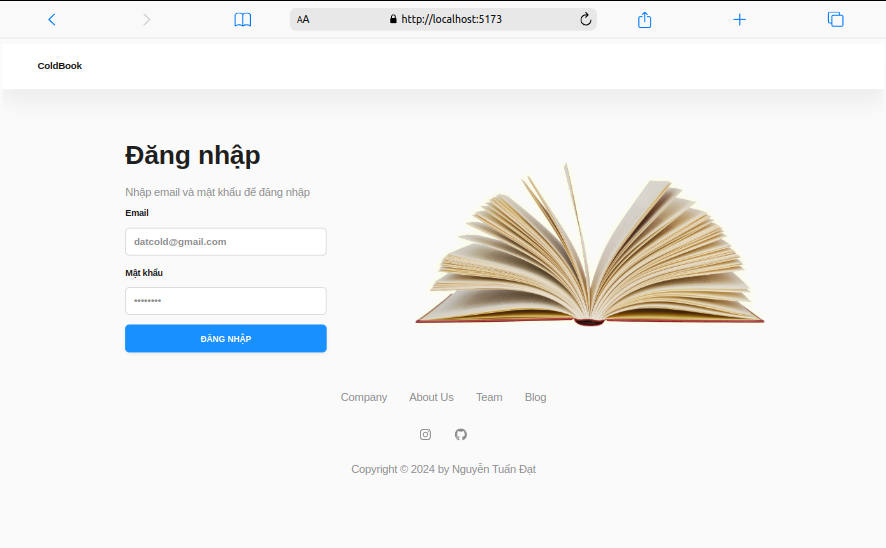
\includegraphics[width=1\textwidth]{report/images/admin/dangnhap.png}
  \caption{Trang đăng nhập}
  % \label{fig:sd-3}
\end{figure}

\phantomsection
\subsubsection{Giao diện trang chủ}
\begin{figure}[H]
  \centering
  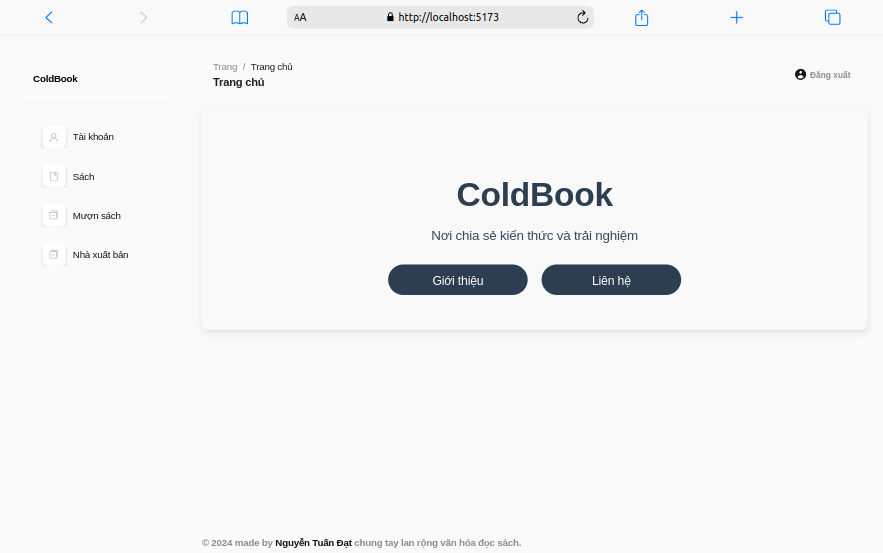
\includegraphics[width=1\textwidth]{report/images/admin/trangchu.png}
  \caption{Trang chủ}
  % \label{fig:sd-3}
\end{figure}
\phantomsection
\subsubsection{Giao diện quản lý tài khoản đọc giả}
\begin{figure}[H]
  \centering
  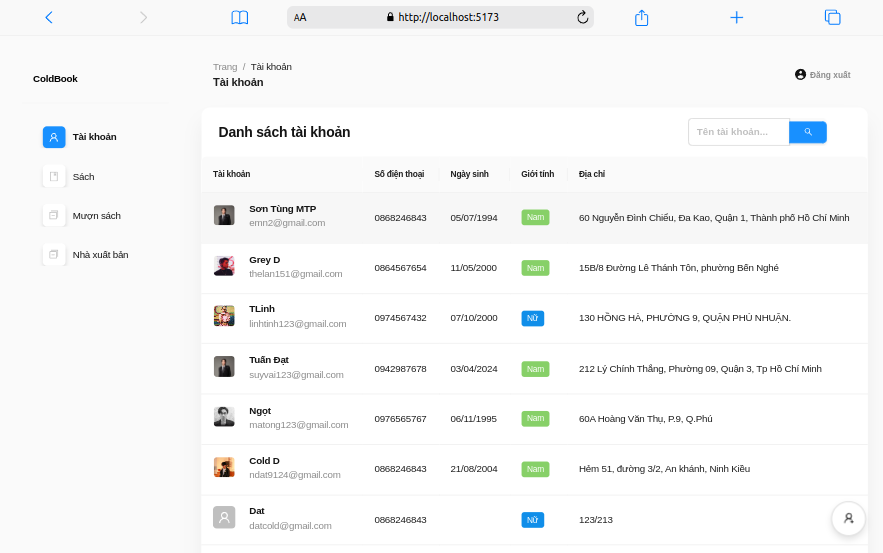
\includegraphics[width=1\textwidth]{report/images/admin/taikhoan.png}
  \caption{Trang quản lý tài khoản đọc giả}
  % \label{fig:sd-3}
\end{figure}
\phantomsection
\subsubsection{Giao diện chỉnh sửa thông tin đọc giả}
\begin{figure}[H]
  \centering
  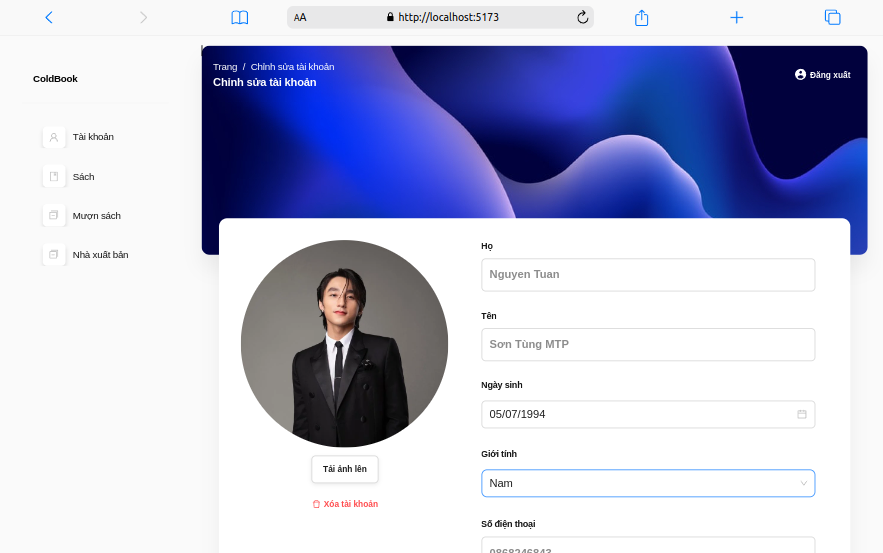
\includegraphics[width=1\textwidth]{report/images/admin/taikhoan_detail.png}
  \caption{Trang chỉnh sửa thông tin đọc giả}
  % \label{fig:sd-3}
\end{figure}
\phantomsection
\subsubsection{Giao diện quản lý sách}
\begin{figure}[H]
  \centering
  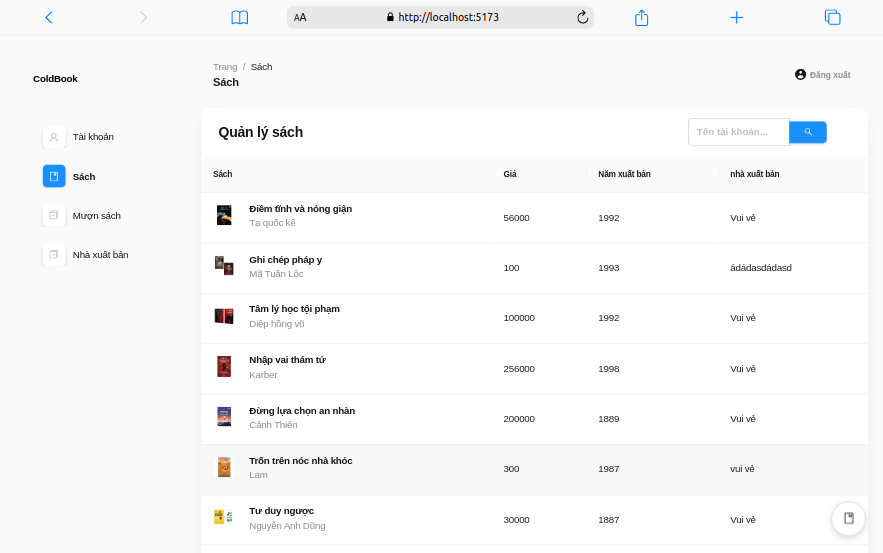
\includegraphics[width=1\textwidth]{report/images/admin/sach.png}
  \caption{Trang quản lý sách}
  % \label{fig:sd-3}
\end{figure}
 
\phantomsection
\subsubsection{Giao diện chỉnh sửa thông tin sách}
\begin{figure}[H]
  \centering
  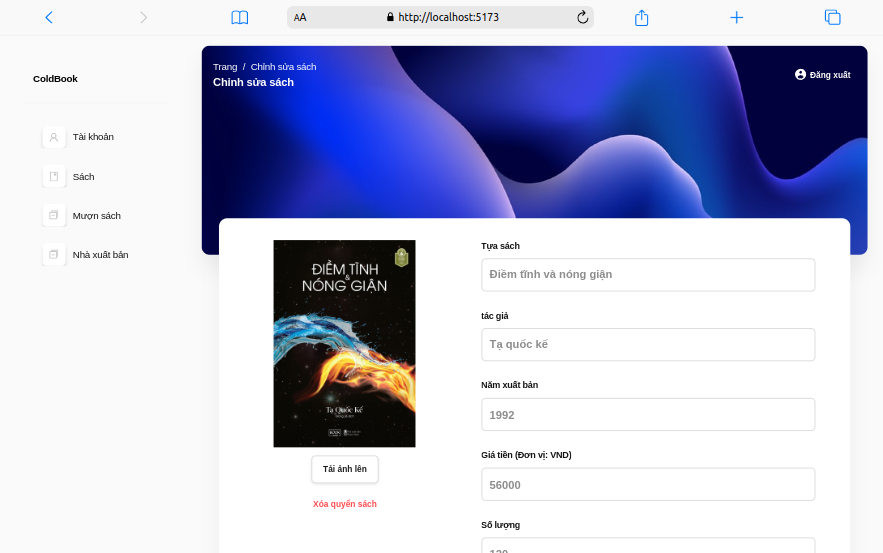
\includegraphics[width=1\textwidth]{report/images/admin/sach_detail.png}
  \caption{Trang chỉnh sửa thông tin sách}
  % \label{fig:sd-3}
\end{figure}
 
\phantomsection
\subsubsection{Giao diện quản lý nhà xuất bản}
\begin{figure}[H]
  \centering
   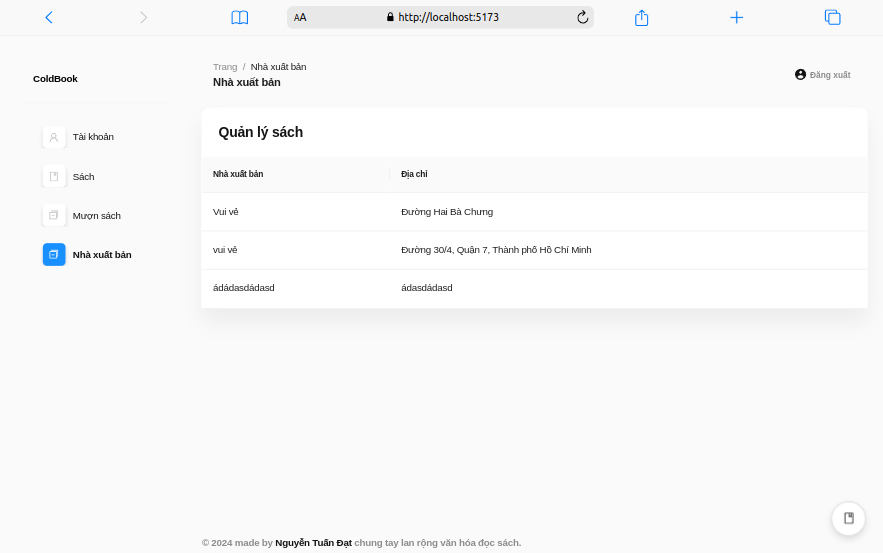
\includegraphics[width=1\textwidth]{report/images/admin/nhaxuatban.png}
  \caption{Trang quản lý nhà xuất bản}
  % \label{fig:sd-3}
\end{figure}


\phantomsection
\subsubsection{Giao diện chỉnh sửa thông tin nhà xuất bản}
\begin{figure}[H]
  \centering
   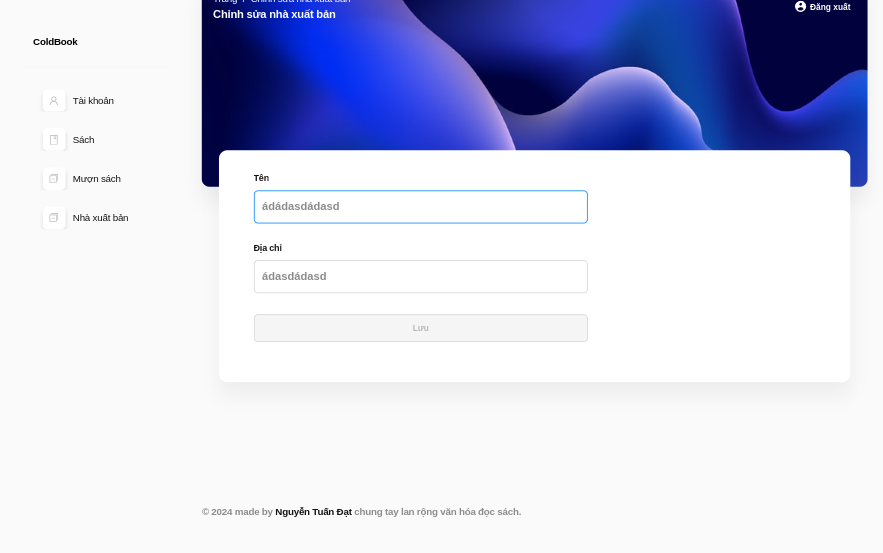
\includegraphics[width=1\textwidth]{report/images/admin/nhaxuatban_detail.png}
  \caption{Trang chỉnh sửa thông tin nhà xuất bản}
  % \label{fig:sd-3}
\end{figure}

\phantomsection
\subsubsection{Giao diện quản lý hóa đơn mượn sách}
\begin{figure}[H]
  \centering
   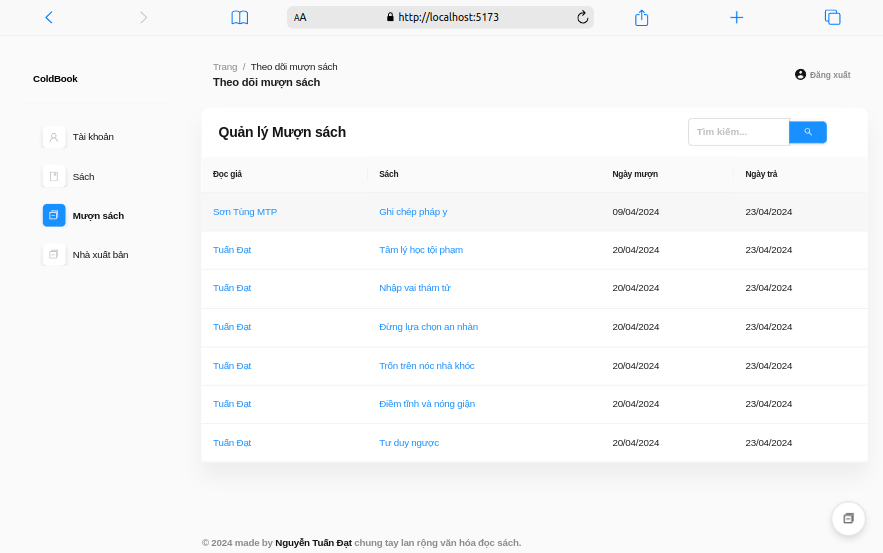
\includegraphics[width=1\textwidth]{report/images/admin/muonsach.png}
  \caption{Trang quản lý sách}
  % \label{fig:sd-3}
\end{figure}


\phantomsection
\subsection{Giao diện của đọc giả}
\setcounter{subsubsection}{0}


\phantomsection
\subsubsection{Giao diện đăng nhập}
\begin{figure}[H]
  \centering
  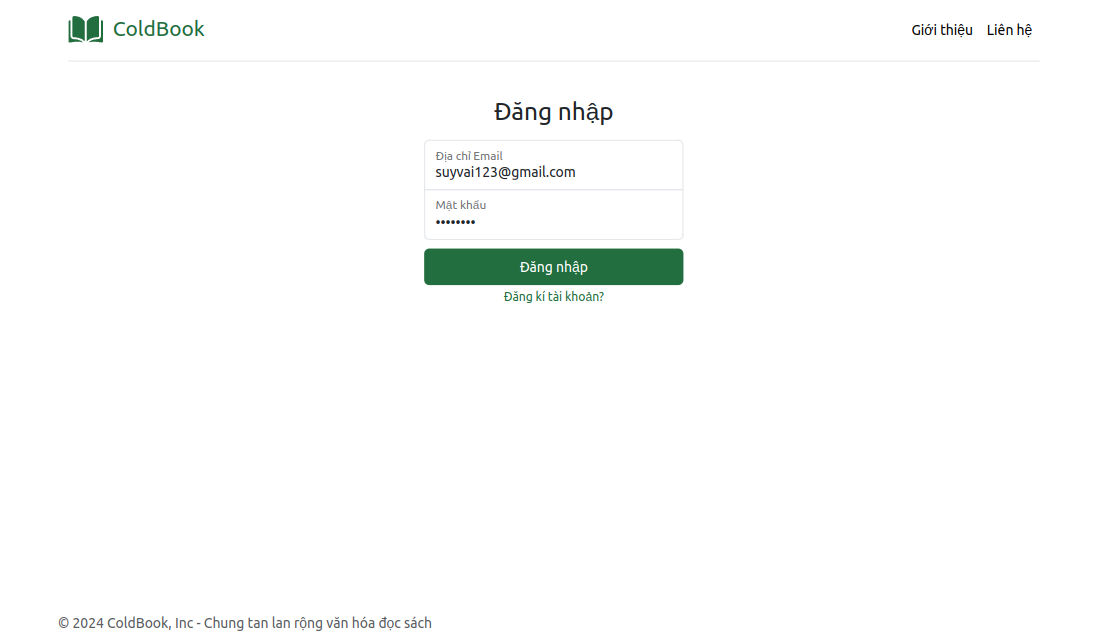
\includegraphics[width=1\textwidth]{report/images/client/c_dangnhap.png}
  \caption{Trang đăng nhập}
  % \label{fig:sd-3}
\end{figure}
\phantomsection
\subsubsection{Giao diện đăng ký}
\begin{figure}[H]
  \centering
  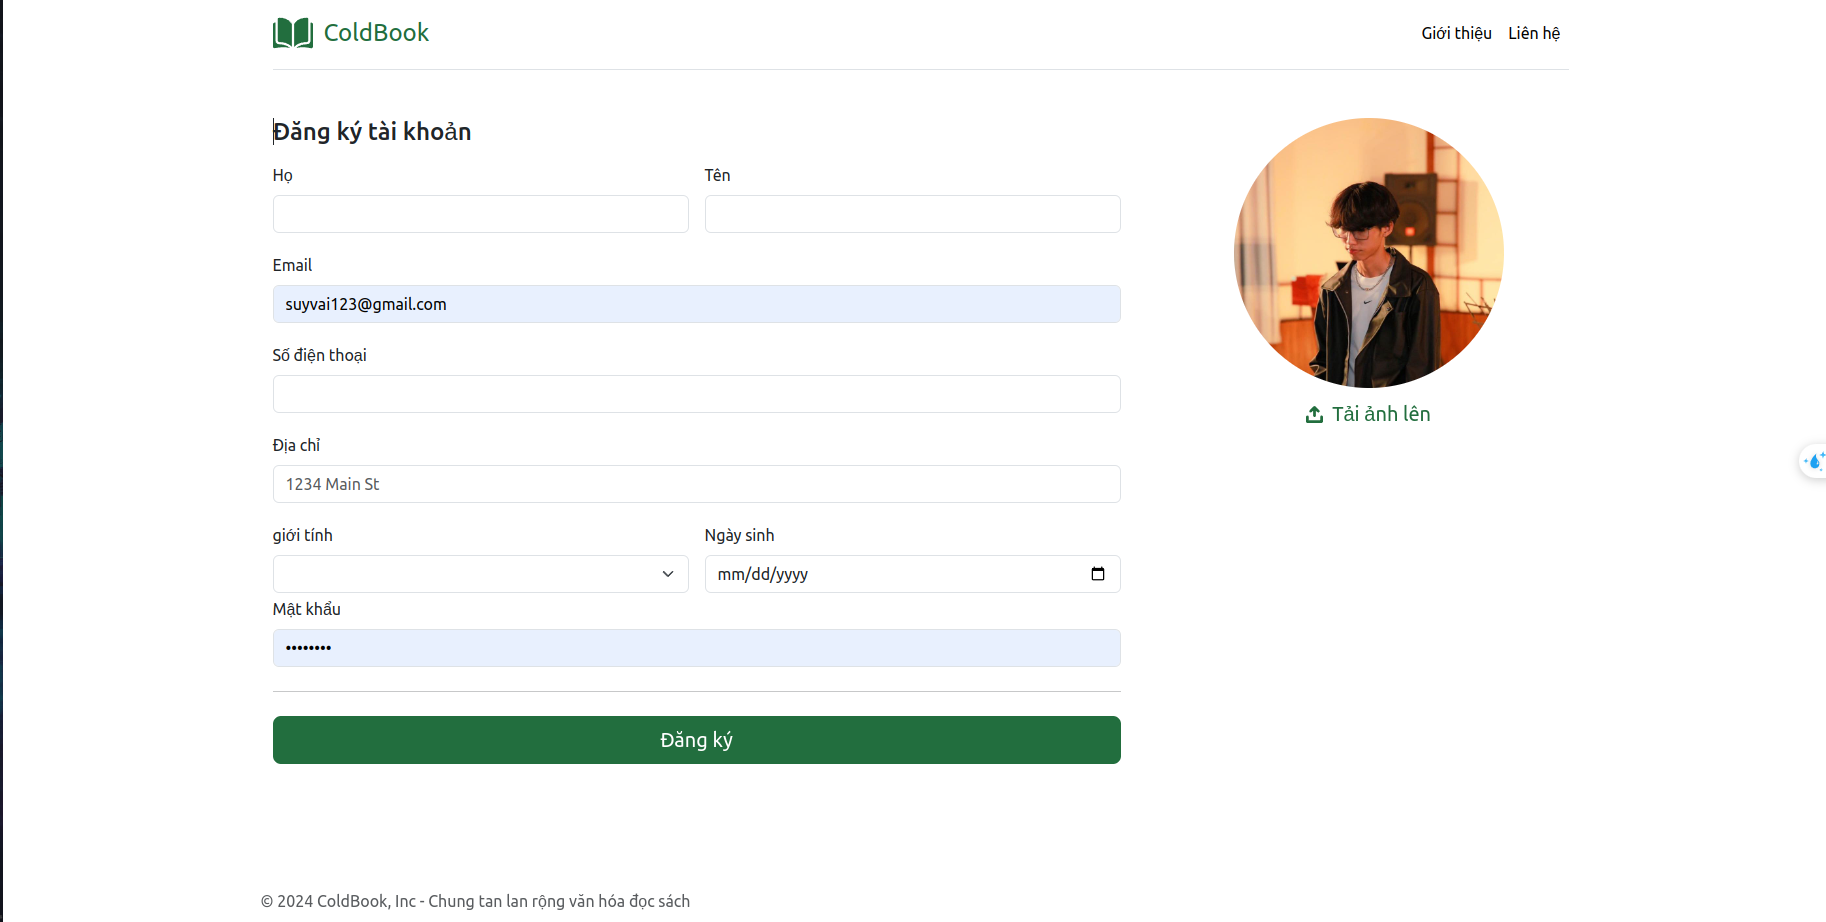
\includegraphics[width=1\textwidth]{report/images/client/c_dangky.png}
  \caption{Trang đăng ký}
  % \label{fig:sd-3}
\end{figure}
\phantomsection
\subsubsection{Giao diện trang chủ}
\begin{figure}[H]
  \centering
  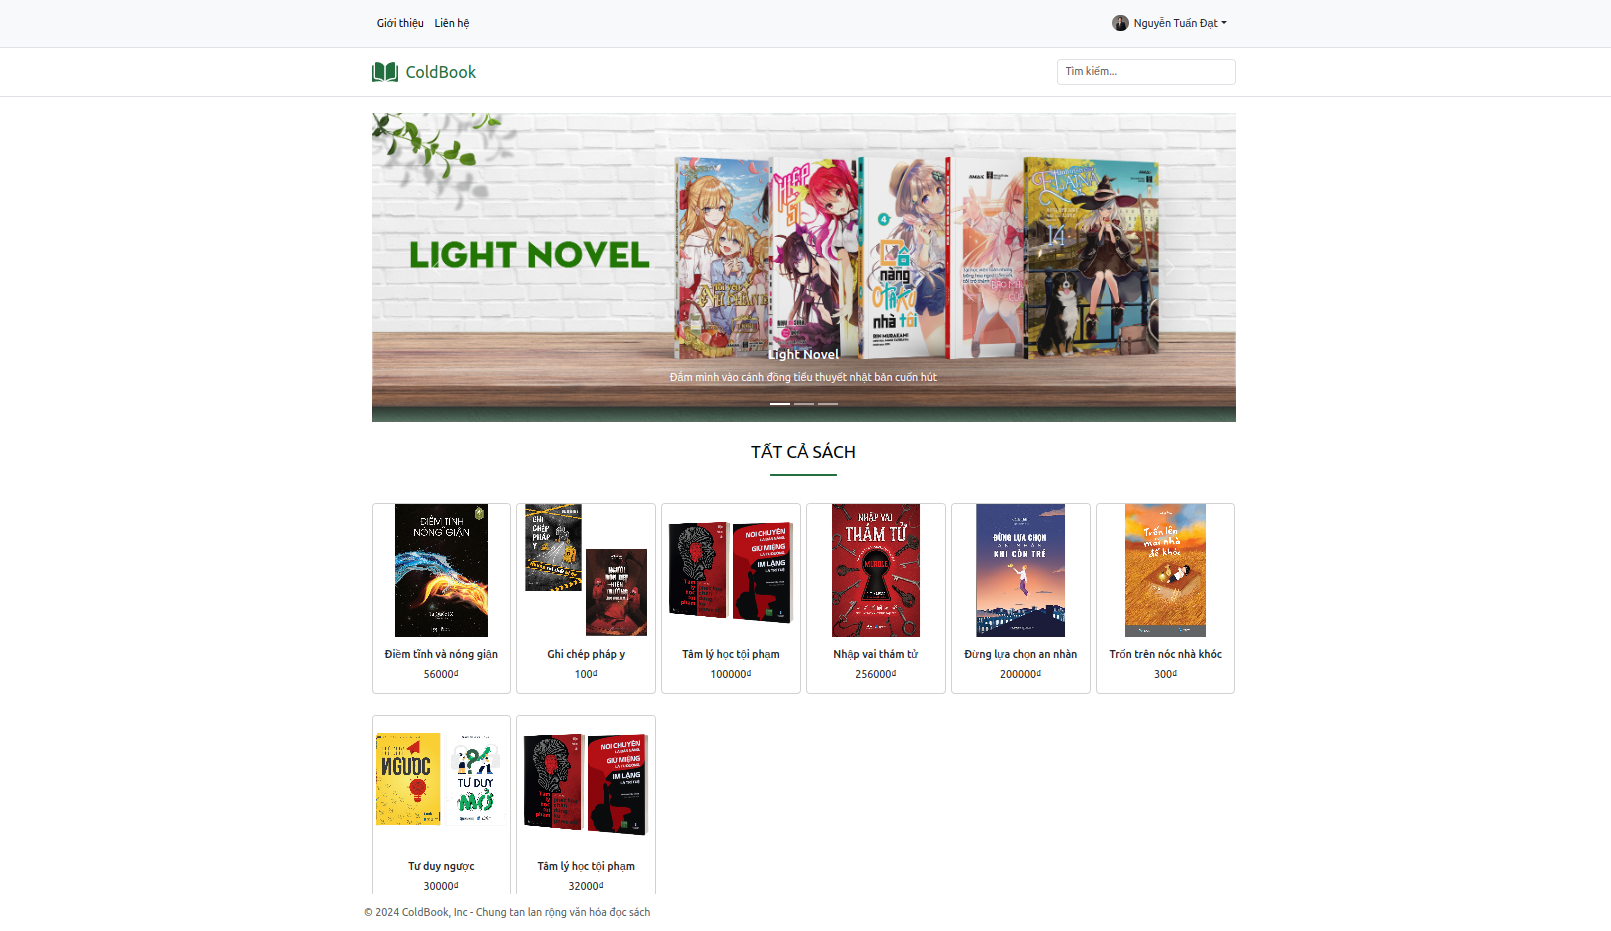
\includegraphics[width=1\textwidth]{report/images/client/c_trangchu.png}
  \caption{Trang chủ}
  % \label{fig:sd-3}
\end{figure}
\phantomsection
\subsubsection{Giao diện mô tả chi tiết sách}
\begin{figure}[H]
  \centering
  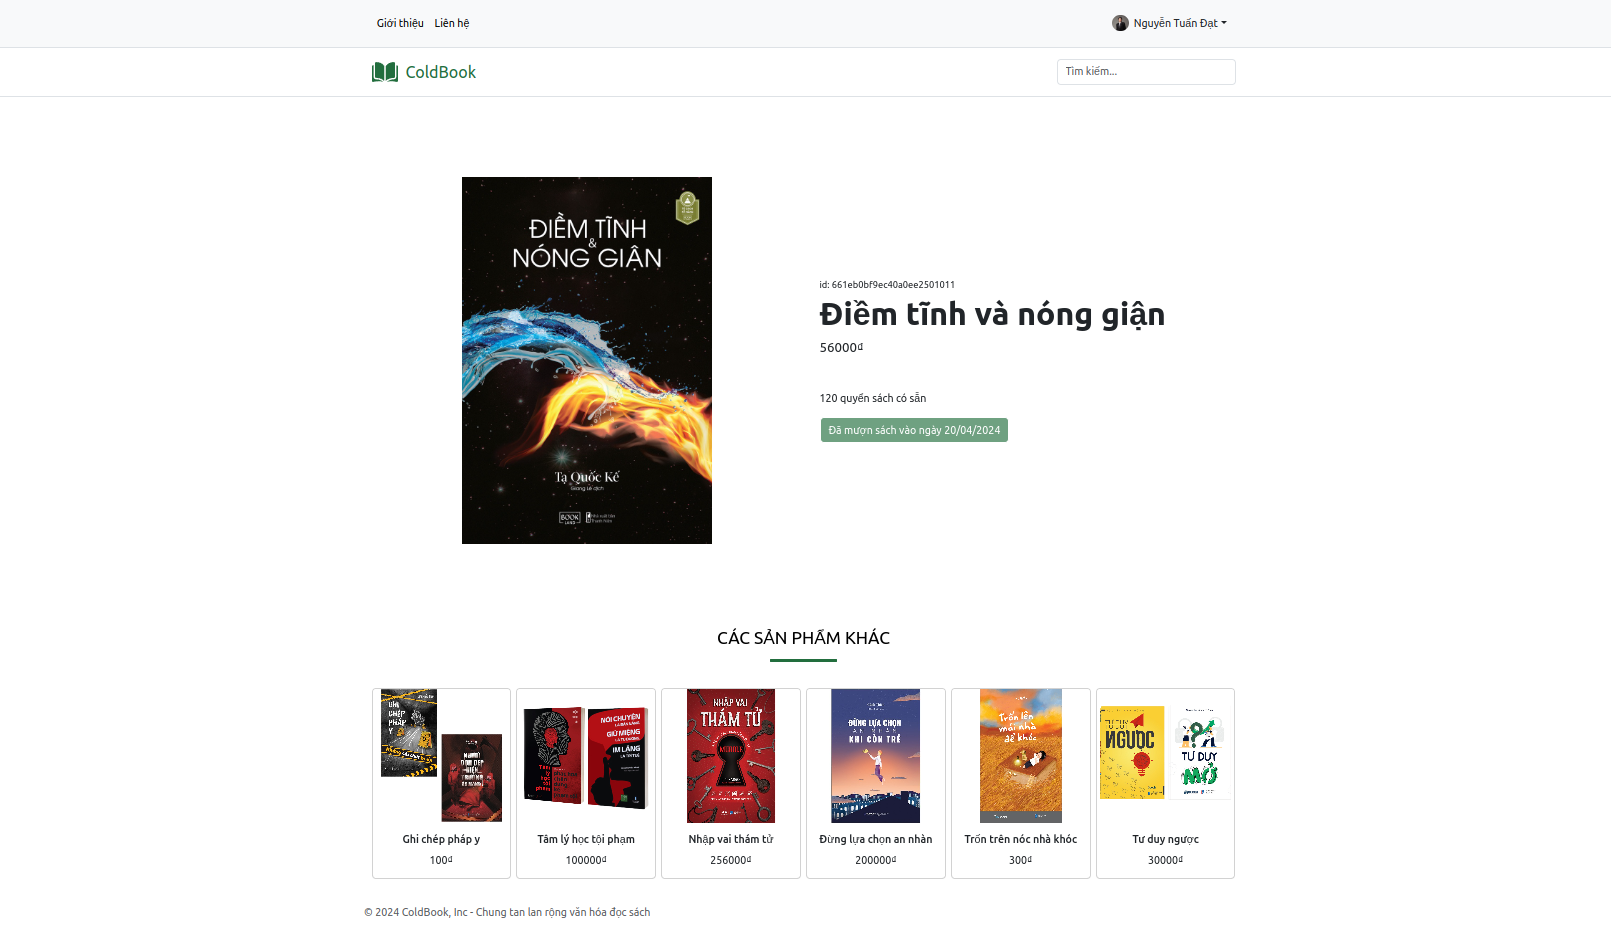
\includegraphics[width=1\textwidth]{report/images/client/c_sach_detail.png}
  \caption{Trang mô tả chi tiết sách}
  % \label{fig:sd-3}
\end{figure}
\phantomsection
\subsubsection{Giao diện lịch sử mượn sách}
\begin{figure}[H]
  \centering
  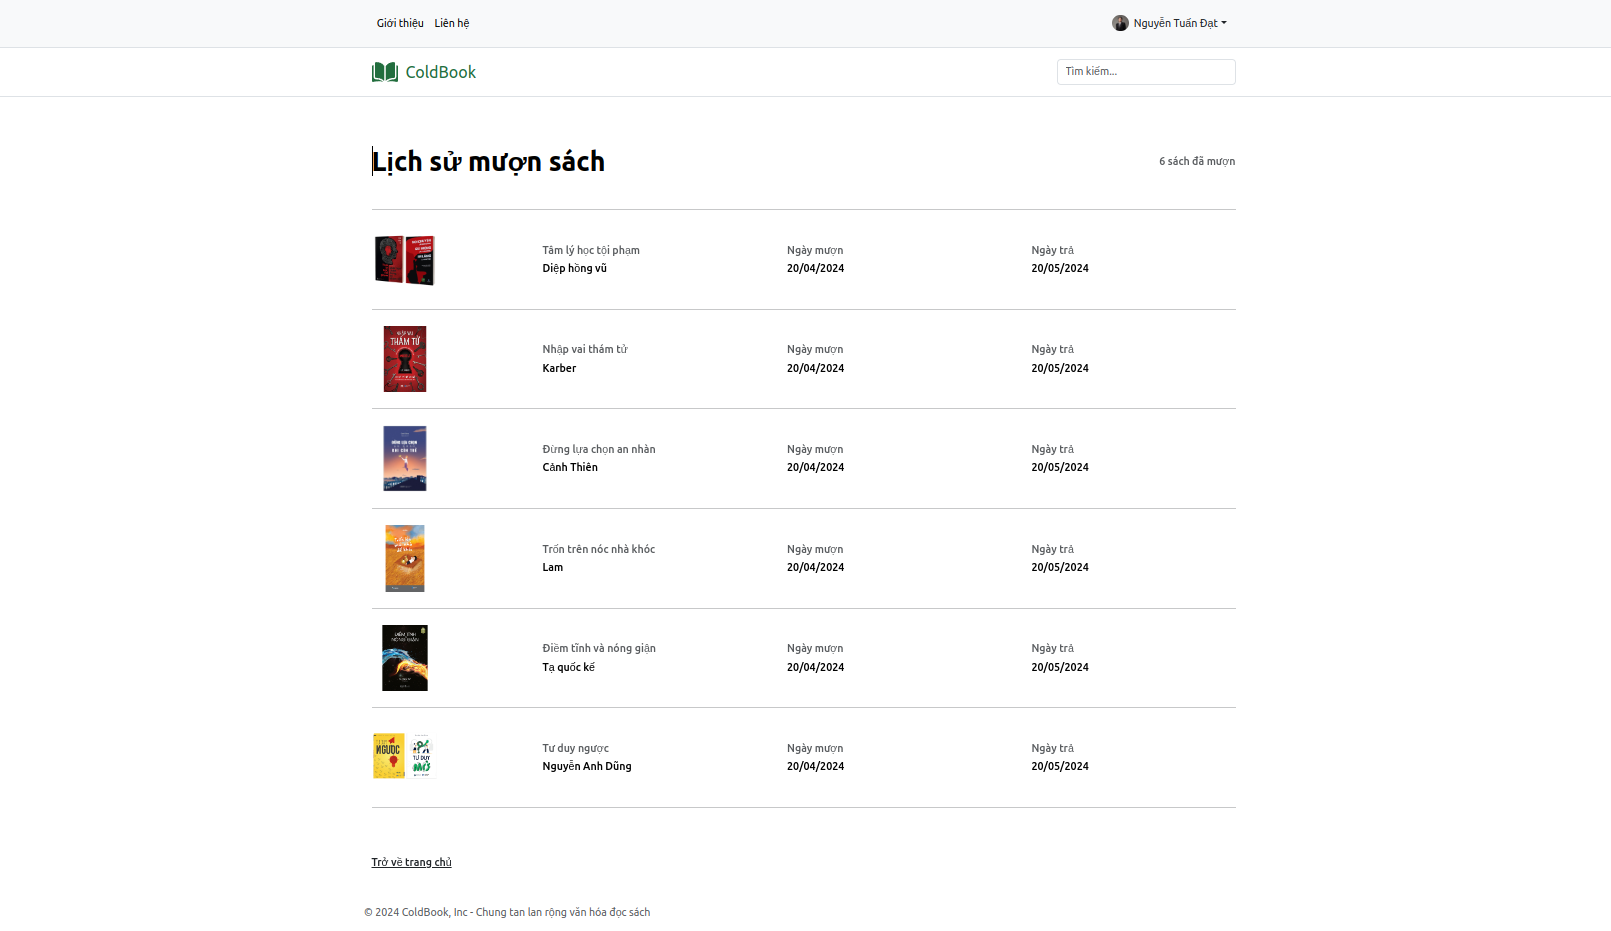
\includegraphics[width=1\textwidth]{report/images/client/c_lichsumuonsach.png}
  \caption{Trang lịch sử mượn sách}
  % \label{fig:sd-3}
\end{figure}
\phantomsection
\subsubsection{Giao diện chỉnh sửa thông tin cá nhân}
\begin{figure}[H]
  \centering
  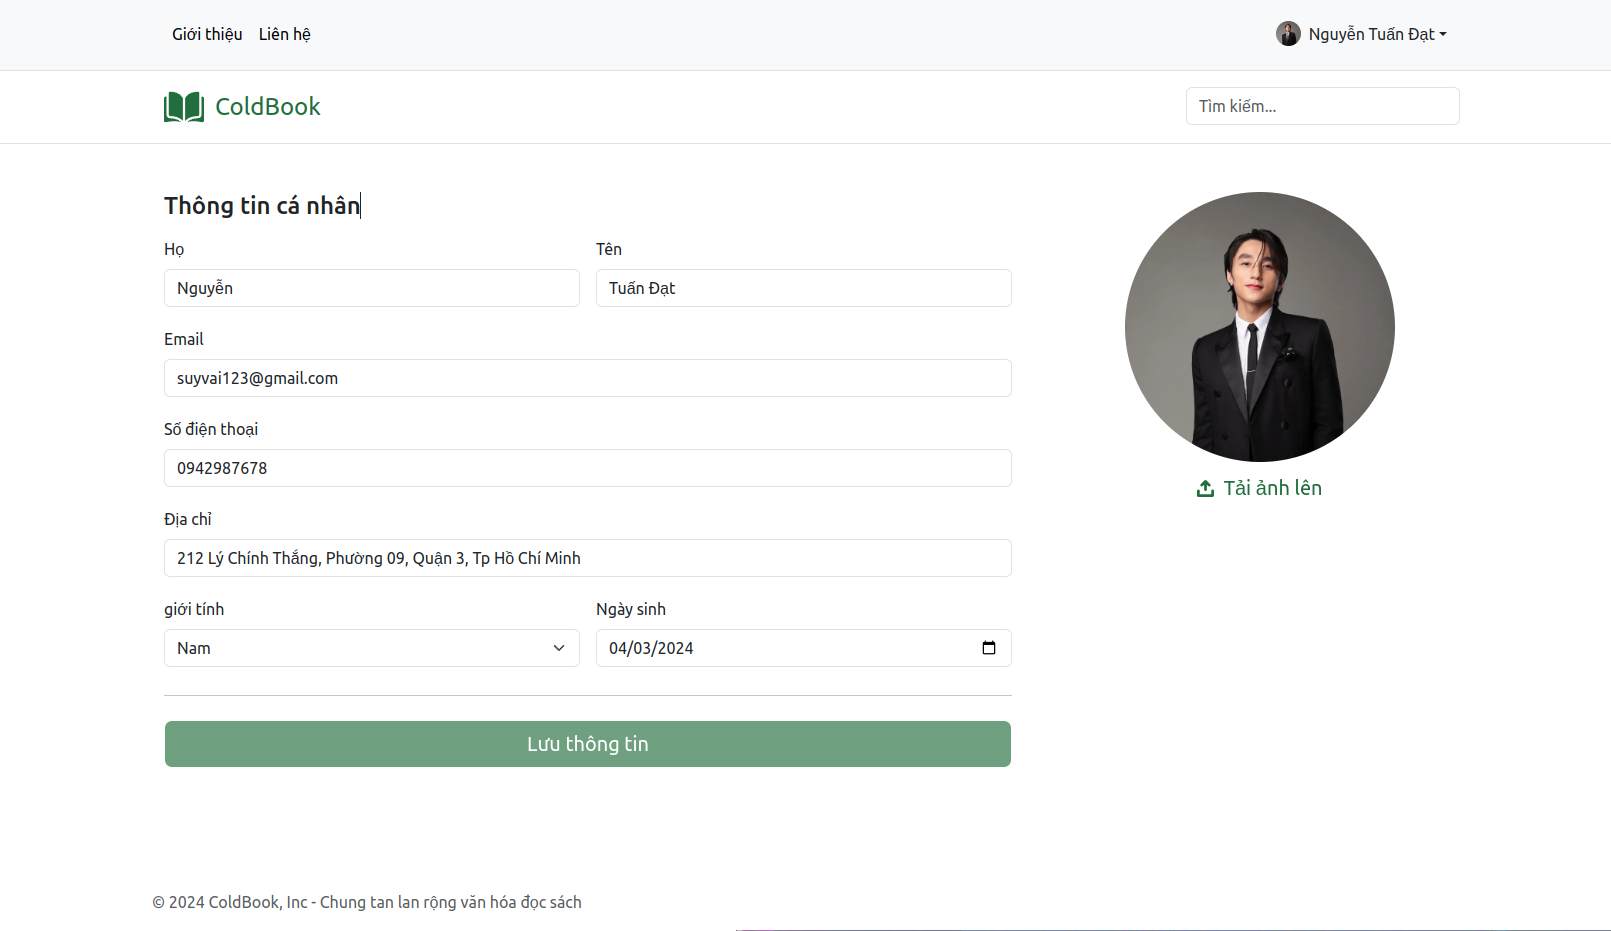
\includegraphics[width=1\textwidth]{report/images/client/c_thongtincanhan.png}
  \caption{Trang chỉnh sửa thông tin cá nhân}
  % \label{fig:sd-3}
\end{figure}
\phantomsection
\subsubsection{Giao diện giới thiệu cửa hàng}
\begin{figure}[H]
  \centering
  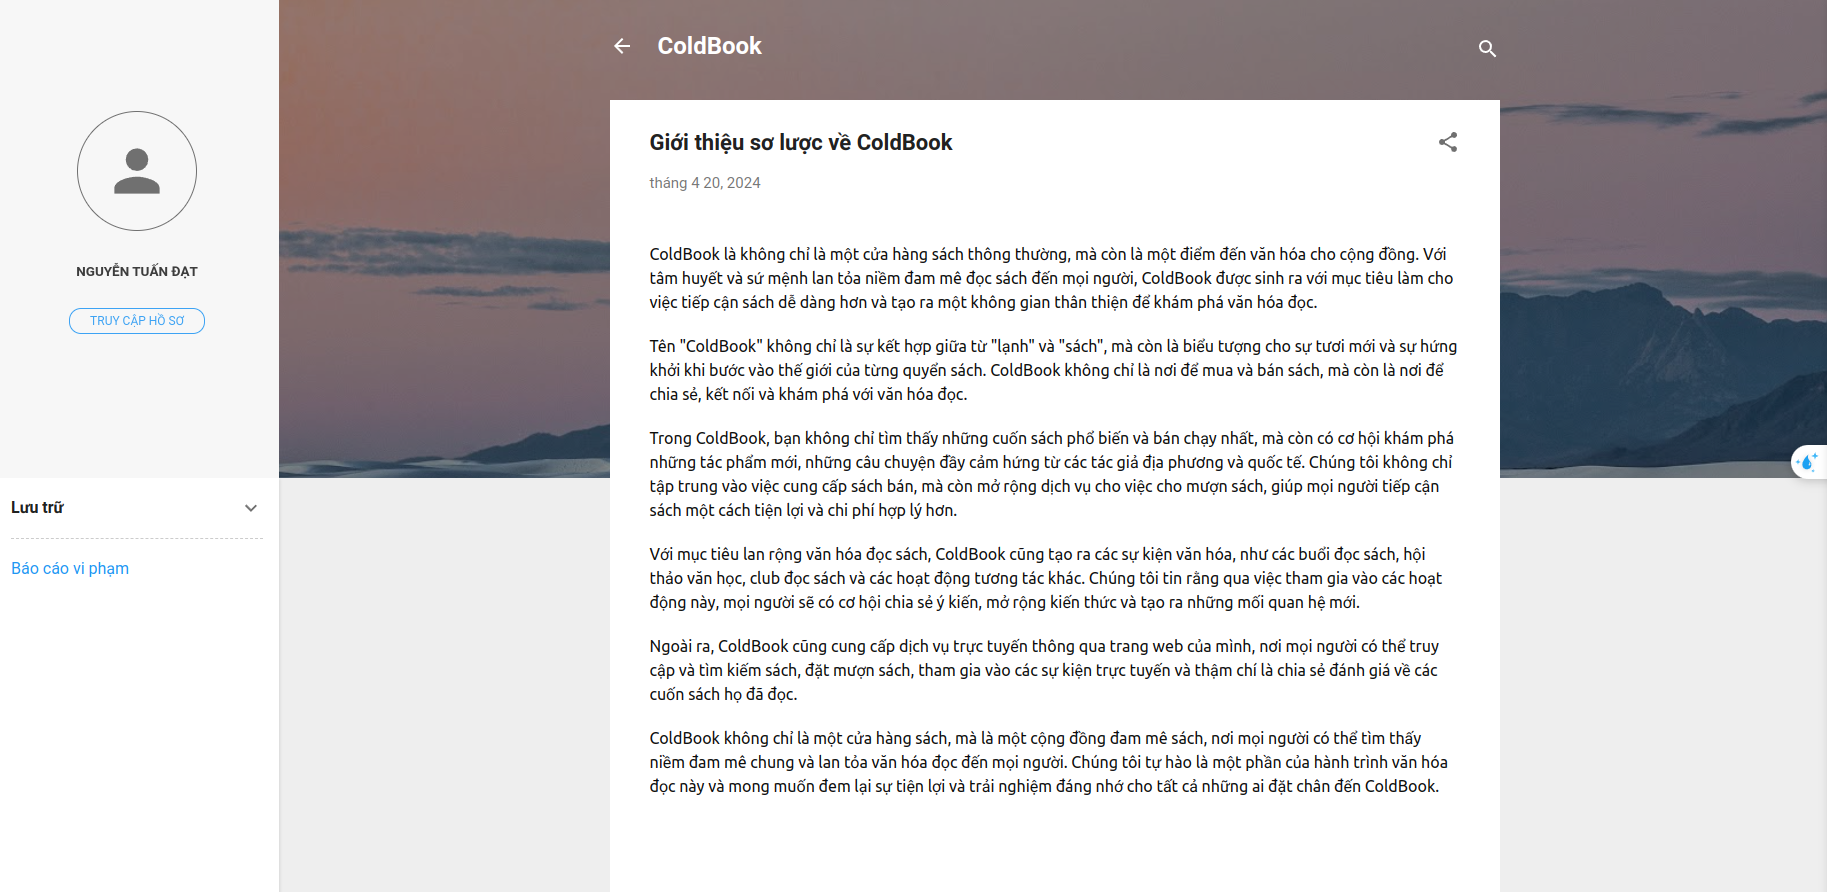
\includegraphics[width=1\textwidth]{report/images/client/c_lienhe.png}
  \caption{Trang giới thiệu của hàng}
  % \label{fig:sd-3}
\end{figure}
\phantomsection
\subsubsection{Giao diện tìm kiếm sách}
\begin{figure}[H]
  \centering
  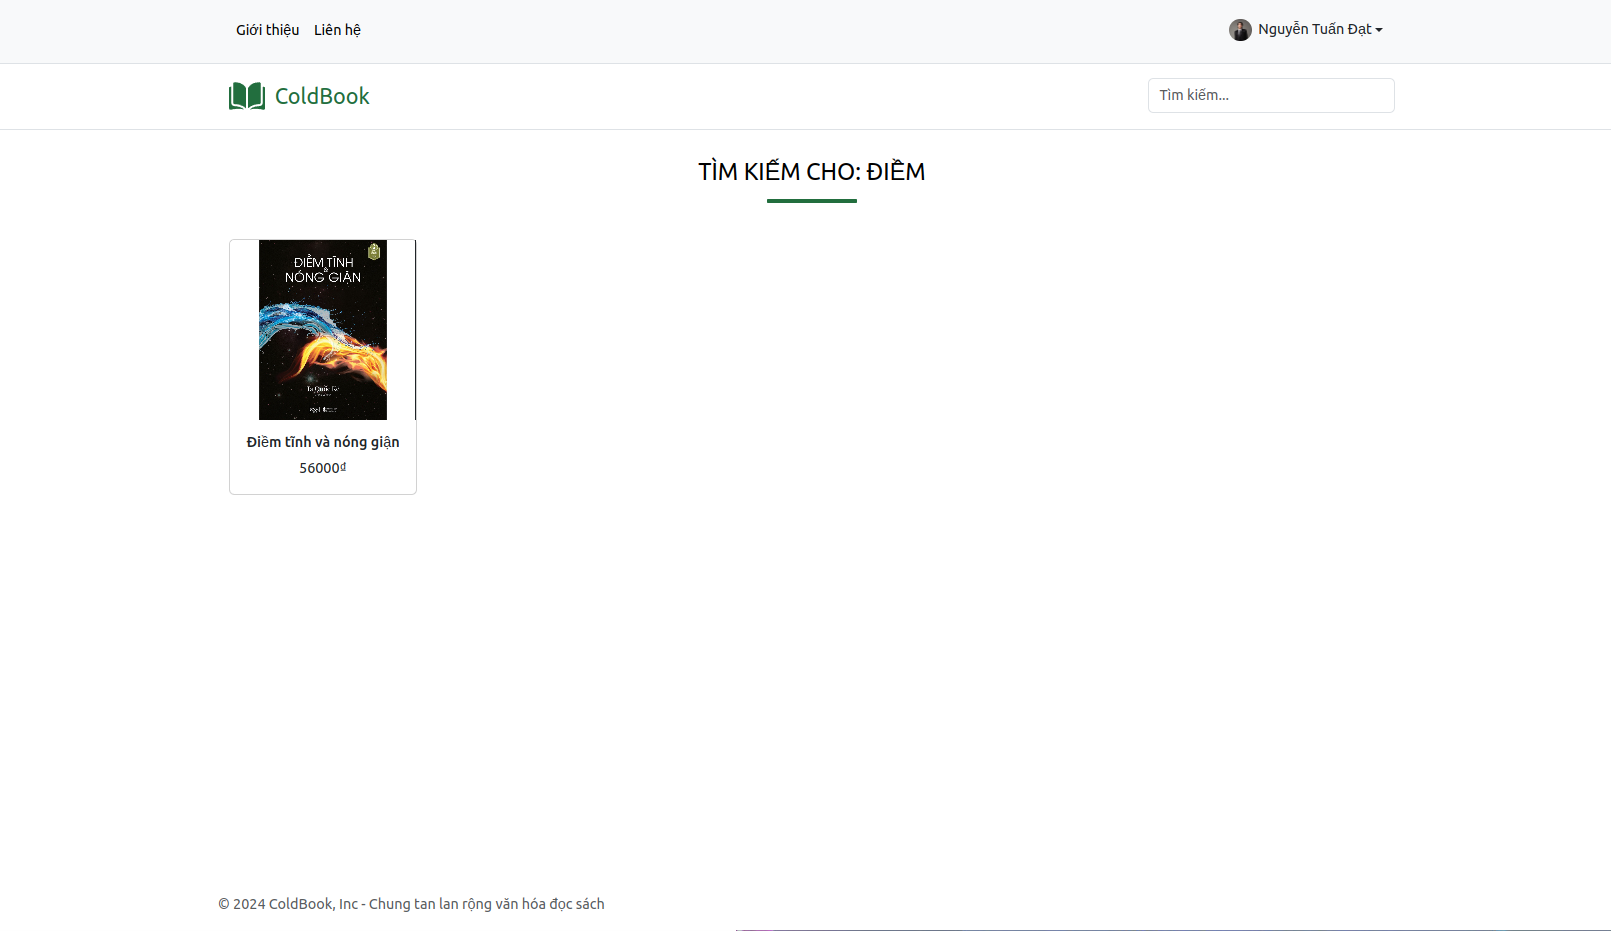
\includegraphics[width=1\textwidth]{report/images/client/c_timkiem.png}
  \caption{Trang tìm kiếm sách}
  % \label{fig:sd-3}
\end{figure}










\phantomsection
\setsection{Chương 5: Kết luận và hướng phát triển}
\setcounter{section}{5}
\setcounter{subsection}{0}

\phantomsection

\subsection{Kết quả đạt được}
Về mặt thực tiễn: Đồ án đã giải quyết thách thức ban đầu bằng cách cung cấp một giải pháp cho việc quản lý và theo dõi mượn sách, mang lại thuận lợi cho người quản lý và đọc giả trong việc tìm kiếm sách.
\par
Về mặt nội dung: Đề tài "Website cửa hàng sách" đã được thiết kế với các chức năng linh hoạt để đáp ứng nhu cầu sử dụng của người dùng. Sử dụng công nghệ Mongoose để quản lý dữ liệu, Bootstrap 5 và Ant Design để tạo giao diện thân thiện và hấp dẫn hơn, kết hợp JWT để bảo vệ tính xác thực của người dùng, cùng với các công nghệ khác để tạo ra một trang web hoàn chỉnh.
\par
Về chức năng: Tất cả các chức năng cơ bản đã được hoàn thiện, đáp ứng đầy đủ nhu cầu của người dùng.


\subsection{Hạn chế}
Do thời gian thực hiện đề tài hạn chế, không có đủ thời gian để thêm một số chức năng và tùy chỉnh để cải thiện trải nghiệm người dùng, bao gồm chức năng quên mật khẩu và tùy chỉnh giao diện như chế độ sáng/tối và đa ngôn ngữ.


\phantomsection

\subsection{Hướng phát triển}
Để tối ưu hóa trải nghiệm của người dùng và tăng tính hiệu quả của trang web, có một số hướng phát triển tiềm năng như sau:

\begin{itemize}[label={+}]
          \item Thêm chức năng mua sách, quản lý hóa đơn và phương thức thanh toán: Đáp ứng nhu cầu của người dùng muốn mua sách để tiện lợi hơn trong việc đọc sách.
          \item Phân loại sách: Thêm tính năng phân loại sách theo thể loại trong cơ sở dữ liệu, giúp người dùng tìm kiếm và lựa chọn sách dễ dàng hơn theo thể loại và giá tiền.
          \item Tùy chỉnh giao diện: Cung cấp khả năng tùy chỉnh giao diện cho người dùng, bao gồm chế độ sáng/tối và đa ngôn ngữ, nhằm tối ưu hóa trải nghiệm người dùng.
          \item Thêm chức năng thống kê cho trang quản lý: Cung cấp các báo cáo và thống kê liên quan đến hoạt động của trang web để người quản lý có thể đánh giá hiệu suất và tối ưu hóa quản lý.
          \item Thêm phần đánh giá cho mỗi quyển sách: Cho phép người đọc đánh giá và chia sẻ ý kiến về các quyển sách, giúp người dùng có cái nhìn tổng quan về chất lượng và sự phong phú của nội dung sách.
        \end{itemize}
\phantomsection
\setsection{Đường dẫn đến github dự án}
\setcounter{section}{6}
\setcounter{subsection}{0}


\begin{enumerate}
    \item \textbf{BackEnd}: \url{https://github.com/dattamlong/CT499-03-BTL}
    \item \textbf{FontEnd-Admin}: \url{https://github.com/dattamlong/CT449-Admin-Vue}
    \item \textbf{FontEnd-Client}: \url{https://github.com/dattamlong/CT499-Client-Vue}
\end{enumerate}






\phantomsection
\addcontentsline{toc}{section}{TÀI LIỆU THAM KHẢO}
\renewcommand{\refname}{TÀI LIỆU THAM KHẢO}
\markright{Tài liệu tham khảo}
\bibliographystyle{IEEEtran}
\bibliography{reference}
\end{document}
